\documentclass[a4paper,10pt]{article}
\usepackage[utf8]{inputenc}
\usepackage{graphicx}
\usepackage{booktabs}
\usepackage{longtable}
\usepackage{rotating}
\usepackage{subfigure}
\usepackage{multirow}
\usepackage{amssymb}
\usepackage{indentfirst}
\usepackage{float}
\usepackage{listings}
\usepackage{url}
\usepackage{cite}
\usepackage{amsmath}
\usepackage{xcite} % Cite stuff from the main text
\usepackage{xr} % automatic cross-referencing
\usepackage[authoryear,round]{natbib}
\bibliographystyle{apalike}
%%% Supp Mat modifications
\renewcommand\refname{Further References}
\externaldocument{FMDV_AMERICA}
\externalcitedocument[M-]{FMDV_AMERICA}
\renewcommand{\thesubfigure}{(\Alph{subfigure})}
\renewcommand{\thetable}{S\arabic{table}}   
\renewcommand{\thefigure}{S\arabic{figure}}

%%%% XML syntax highlighting
\usepackage{color}
\definecolor{gray}{rgb}{0.4,0.4,0.4}
\definecolor{darkblue}{rgb}{0.0,0.0,0.6}
\definecolor{cyan}{rgb}{0.0,0.6,0.6}

\lstset{
  basicstyle=\ttfamily,
  columns=fullflexible,
  showstringspaces=false,
  commentstyle=\color{gray}\upshape
}

\lstdefinelanguage{XML}
{
  morestring=[b]",
  morestring=[s]{>}{<},
  morecomment=[s]{<?}{?>},
  stringstyle=\color{black},
  identifierstyle=\color{darkblue},
  keywordstyle=\color{cyan},
  morekeywords={xmlns,version,type}% list your attributes here
}

%%%%%
\topmargin 0.0cm
\oddsidemargin 0.5cm
\evensidemargin 0.5cm
\textwidth 16cm
\textheight 21cm
\pagestyle{myheadings}
%%%%%
%opening
\title{Text S2 -- Supplementary information to ``Spatio-temporal Dynamics of Foot-and-Mouth Disease Virus in South America''}
\author{
Luiz Max Carvalho, Nuno Rodrigues Faria, Andres Perez,
Marc A. Suchard,\\ 
Philippe Lemey, Waldemir de Castro Silveira,\\
Andrew Rambaut and Guy Baele
}

\date{August, 2019}
\begin{document}

\maketitle

\section*{Data collection and curation}

\subsection*{Sequence data}

In Tables~\ref{stab:sequences_A} and~\ref{stab:sequences_O} we provide the GenBank accession numbers, date and country of collection of all sequences used in this study.

\subsection*{Livestock trade data}

One of the main contributions of this study lies in exploring the association between the trade of cattle, pigs and sheep and viral diffusion using a statistically sound approach that enables us to test evolutionary hypotheses concerning the influence of these predictors on viral spread~\citep{M-Lemey2014}. %GB: cite Lemey et al. 2014
In this text we provide some additional exploratory plots of the covariate data.
In Figure~\ref{sfig:prod}, we show the time series of livestock production among the studied countries for a time frame of over $50$ years, illustrating that the production of cattle is much larger than that of any other livestock. %GB: I think that a simple line plot, connecting the dots would make the figure more clear than drawing a straight regression line through the dots
Perhaps more importantly, while pigs and cattle production maintain a trend of positive growth throughout the second half of the twentieth century, sheep production shows a decline after $1990$.
Spatially, the trade of all three livestock is rather different, as shown in Figure~\ref{sfig:tradenets}. %GB: this figure is not very clear; would it not be better to use dot matrices, with the size of the dots proportional to the trade intensity? Or perhaps use the existing figure(s) but play with the width of the different arrows according to trade intensity?
% LM: I strongly disagree. But then again I'm biased; this took me a long time to code up and is clear enough to me. I'll wait to see whether this bothers others too.
The cattle trade network is more connected, while the pig and sheep trade networks are considerably more sparse.
Further, the pig network presents a clear regional pattern, with two sub-networks. %GB: clearly illustrate these two networks on the figure?
%LM: Good idea. Will see what I can do. Later.

Temporally, overall trade shows remarkably different trends depending on the livestock analysed.
While cattle trade shows a positive trend, pig trade is mostly stable over time and all other livestock considered show a declining trend.
The FAO trade matrix is sometimes inconsistent, i.e. sometimes the exports from country $i$ to country $j$ do not correspond to the imports into country $j$ from country $i$.
In cases like these we have picked the largest value for a given year and pair of countries $i$ and $j$.

\subsection*{Vaccination and case data}

We obtained the number of vaccine doses distributed in a given country in a given year starting from 1986 and ending in 2010 and divided this total by the number of live cattle produced per country and year.
We could not find information for the years of 1991 and 1996 and resorted to manually imputing the missing values for these years by taking the arithmetic mean of the two adjacent years.
This indicator is only a proxy for vaccination in the continent since (i) not all vaccines administered protect against all serotypes and (ii) cattle are not the only susceptible livestock.
We argue our choices are justified however, because (i) most vaccine doses were actually protective against all 3 serotypes (trivalent) and (ii) cattle are by far the most numerous livestock in South America and their vaccination is mandatory across all affected countries.

We obtained a temporal measure of vaccination by computing the average across the nine countries per year.
As a measure of dispersion, we employed the standard error, multiplied by the 95\% quantile of a Student t distribution with either $\nu = 8 -1 = 7$ or $\nu = 9-1 = 8$ degrees of freedom ($2.36$ and $2.31$, respectively).
We show these vaccination time series in Figure~\ref{sfig:vaccination_temporal}, where it can be observed that there is substantial heterogeneity across countries in terms of temporal vaccination pattern.

\section*{Analysis}

\subsection*{Maximum likelihood phylogenies and root-to-tip divergences}

In order to preliminarily assess whether the data sets used in this study contain evidence of clock-like evolution, we construct unrooted phylogenies using the maximum-likelihood procedures implemented in PhyML 3.0~\citep{M-Guindon2003} under a GTR model~\citep{M-Tavare1986} of sequence evolution with gamma-distributed site rate heterogeneity. %GB: cite Yang 1994 or 1996
We root the trees at the branch -- as well as a position along it -- that minimises the sum of squared residuals of the linear regression of root-to-tip divergences (RDV) on the sampling times.
For this last step, we use the routines in the program TempEst~\citep{M-Rambaut2016}.
The resulting trend lines presented in Figure~\ref{sfig:root-to-tip} are consistent with clock-like evolution, despite considerable variation between lineages, which we address later in the paper using relaxed molecular clocks.

An initial RDV analysis indicated that some sequences collected for serotype O had evolutionary divergences incompatible with their dates, and these were excluded from subsequent analyses.
The excluded sequences are listed in Table~\ref{stab:exclseqs}.

\begin{table}[H]
\caption{\textbf{Sequences excluded from analysis.}
Serotype O sequences that displayed genetic divergences inconsistent with their sampling dates were excluded from analysis.
These were sequences with older dates that presented a much higher than expected number of mutations.
}
\begin{center}
\begin{tabular}{ccccccc}
\toprule
Accession & Year & Country \\      
\midrule
AY593818 & 1958 & Brazil \\
AY593837 & 1963 & Uruguay \\ 
AY593820 & 1964 & Argentina  \\
AY593814 & 1965 & Argentina \\
AY593821 & 1967 & Argentina \\
\bottomrule
\end{tabular}
\end{center}
\begin{flushleft}
\end{flushleft}
\label{stab:exclseqs}
 \end{table}

 
\subsection*{Bayesian Model Selection}

We employed generalised stepping stone sampling (GSS, \citet{M-Baele2016}) to compute (log) marginal likelihoods for six combinations of Markov sequence evolution and molecular clock models. %GB: citation year is wrong, should be 2016
A constant population size coalescent tree prior was used across all combinations. %GB: the main manuscript seemed to suggest that the constant population size model was going to be compared against the Skygrid model using model selection
We used $50$ steps with $250,000$ iterations per step, with the resulting 51 power posteriors spaced according to a Beta($\alpha = 0.3$, 1.0) distribution. %GB: cite Xie et al. 2011 and Baele et al. 2016
Table~\ref{stab:treeclockselection} shows the results of this model selection study to determine the best combination of sequence substitution and molecular clock models for each serotype.

For serotype A, the model combination with the highest (log) marginal likelihood is a GTR sequence evolution model coupled with an uncorrelated relaxed clock assuming an underlying Gamma distribution (UCG), whereas for serotype O the best model combination was GTR and an uncorrelated relaxed clock assuming an underlying log-normal distribution (UCLN).
The quantile inversions for the Gamma relaxed clock model are very compute-intensive and computations for this model took much longer to finish.
In the interest of computational expediency for the large number of subsequent analyses we performed in this paper, we decided to use the UCLN model for serotype A as well.

\begin{table}[!ht]
\caption{\textbf{Marginal likelihoods for combinations of sequence evolution (Markov) and molecular clock models.}
We used the generalised stepping stone (GSS) from~\citep{M-Baele2016} to compute (log) marginal likelihoods using a constant population size coalescent tree prior.
We compared the HKY and GTR substitution models, in combination with the strict clock and the uncorrelated relaxed clock models assuming either an underlying log-normal distribution (UCLN) or gamma distribution (UCG).
The best fitting model for each serotype is highlighted in bold.
}
\begin{center}
 \begin{tabular}{cclc}
\hline
Serotype & Markov model & Clock model & log marginal likelihood \\
\hline
\multirow{6}{*}{A} & GTR & UCLN & -13649.55 \\
 & GTR & UCG & \textbf{-13619.52} \\
 & GTR & Strict & -13721.67 \\
 & HKY & UCLN & -13668.54 \\
 & HKY & UCG & -13664.53 \\
 & HKY & Strict & -13760.31 \\
 \hline
\multirow{6}{*}{O}& GTR & \multicolumn{1}{l}{UCLN} & \textbf{-9917.44} \\
\multicolumn{1}{l}{} & GTR & \multicolumn{1}{l}{UCG} & -9925.08 \\
\multicolumn{1}{l}{} & GTR & \multicolumn{1}{l}{Strict} & -10085.06 \\
\multicolumn{1}{l}{} & HKY & \multicolumn{1}{l}{UCLN} & -9959.38 \\
\multicolumn{1}{l}{} & HKY & \multicolumn{1}{l}{UCG} & -9955.12 \\
\multicolumn{1}{l}{} & HKY & \multicolumn{1}{l}{Strict} & -10102.83\\
\hline
\end{tabular}
\end{center}
\label{stab:treeclockselection}
\end{table}
\newpage

\subsection*{Temporal analysis -- accounting for preferential sampling}

Since our sample is likely to be biased temporally -- as well as spatially (but see below) --, we employ a population dynamics reconstruction method that allows accommodating the tip sampling structure, as well as the inclusion of temporal covariates~\citep{M-Karcher2019}.
The model of~\cite{M-Karcher2019} assumes sequences are collected according to a Poisson point process with intensity
\begin{equation}
 \label{eq:skytrack}
 \lambda_s(t) = \exp\left( \beta_0 + \beta_1\gamma(t) + \beta_2 f_1(t)  + \beta_2 f_2(t) + \ldots + \beta_P f_P(t) + \left[\delta_2 f_2(t) + \ldots + \delta_P f_P(t) \right]\gamma(t) \right),
\end{equation}
where $\gamma(t)$ is the log population size at time $t$, the $\boldsymbol\beta$ are coefficients, $\mathcal{F} = \{f_1, f_2, \ldots, f_P\}$ are functions of interest and the $\boldsymbol\delta$ control interaction terms, which we do not use here.
Following~\cite{M-Karcher2019}, we consider four models:
\begin{enumerate}
 \item \textbf{Model 0:} ``Naive'' model, in which sampling is not accounted for~\citep{Palacios2015}.
 \item \textbf{Model 1:} Preferential model with $\lambda_s(t) = \exp(\beta_0 + \beta_1\gamma(t))$, denoted $\{\gamma(t)\}$~\citep{M-Karcher2016};
 \item \textbf{Model 2:} Preferential model using $-t$ as a covariate, thus $\lambda_s(t) = \exp(\beta_0 + \beta_1\gamma(t) -\beta_2 t)$, denoted $\{\gamma(t), -t\}$;
 \item \textbf{Model 3:} Preferential model using both $-t$ and $-t^2$ as covariates, thus $\lambda_s(t) = \exp(\beta_0 + \beta_1\gamma(t) -\beta_2 t - \beta_3t^2)$, denoted $\{\gamma(t), -t, -t^2\}$;
\end{enumerate}

These models were fitted using three maximum clade credibility (MCC) trees for each serotype, obtained from three independent chains. %GB: but ideally these 3 MCC trees should be identical, so this could raise some questions %LM: I beg to strongly differ. MCC trees are estimates and hence subject to variation. At this tree size, seeing to identical trees is extremely improbable.
Since results were consistent across MCC trees, we shall discuss only results for one MCC for each serotype.
Complete analyses can be found at~\url{https://github.com/maxbiostat/FMDV_AMERICA/blob/master/CODE/notebooks/BNPR_analysis_covariates.ipynb}.

In order to compare models, we employ (log) marginal likelihoods to compute (log) Bayes factors.
Model 0 does not use sampling data and thus is not directly comparable to the other models.
Models 1 and 2 can be seen as special cases of model 3, with suitably constructed, point-mass priors on the non-shared parameters.
Therefore, we compare models 1, 2 and 3 using the (log) marginal likelihood estimate provided by the underlying integrated nested Laplace approximation (INLA, \cite{Martins2013}), which is computed following~\citet{Hubin2016}.

\subsubsection*{Prior modelling}

% We follow the framework of~\cite{M-Gill2016} in order to incorporate information from temporal predictors into the reconstruction of past (effective) population size.
% This necessitates the specification of priors for the predictor coefficients ($\beta^{\text{Skygrid}}_i, i = 1, \ldots, 13$).
% We assign independent standard normal (Gaussian) priors, $\beta^{\text{Skygrid}}_i \sim \text{Normal}(0, 1)$.
The smoothness of the population trajectory in the Skygrid~\citep{M-Gill2013} %GB: incorrect citation year, should be 2013
and related models is controlled by a precision parameter, $\tau$, which needs to be estimated from the data and thus be given a prior.
The prior usually employed is a Gamma distribution with parameters $\alpha = \beta = 0.001$. 
However, we feel this prior places too much mass on small precisions (which would make estimates noisier) while at the same time allowing rather extreme values, which would artificially inflate confidence.
We instead employ the penalised complexity (PC) prior from~\citet{M-Simpson2017} (pg.14), a density from the Gumbel type II family.
Let $a, b > 0$ be the shape and scale hyperparameters respectively; the probability density function is then
\begin{equation}
 \pi_2(\tau \mid a, b) = ab \cdot \tau^{-a-1}\exp\left(-b\tau^{-a}\right),\: \tau > 0.
\end{equation}
The authors recommend $a = 1/2$ and $b$ to be chosen such that $Pr(1/\sqrt{\tau} > S) = p$, where the value $S$ and the probability $p$ are to be chosen on substantive grounds, such that $b = \ln(p)/S$.
Here we will choose $S = 1$ and $p = 0.1$, which is to say that the prior is constructed such that there is a $10\%$ probability that the standard deviation of the log-population sizes is greater than $1$.
This argument leads to $b = 2.302585$.
This prior has been implemented in BEAST 1.10~\citep{M-Suchard2018} and can be used with the Skygrid model by using the following XML syntax:
\lstset{language=XML}
\begin{center}
\begin{tabular}{c}
\begin{lstlisting}
<gumbelPrior shape="0.5" scale="2.30">
    <parameter idref="skygrid.precision"/>
</gumbelPrior>	
\end{lstlisting}
\end{tabular}
\end{center}
replacing the default XML block.
For the~\textbf{phylodyn} package~\citep{M-Karcher2017}, the PC prior is also implemented in this fork:~\url{https://github.com/maxbiostat/phylodyn}, and can be used by calling~\verb|BNPR(..., pc_prior = TRUE, S, p)| and~\verb|BNPR_PS(..., pc_prior = TRUE, S, p)|.

 
\subsubsection*{Simulations}

In order to understand how the sequence sampling structure of both serotypes (see Figure~\ref{sfig:sampling}) might influence results, we simulated four scenarios for each data set:
\begin{itemize}
 \item[A)] Using the empirical sampling dates, simulate phylogenies under a constant population size with $N_e = 10$;
 \item[B)] Using the empirical sampling dates, simulate phylogenies under an exponential growth model with $N_0 = 10$ and $r = 0.1$;
 \item[C)] Using a regular grid of dates spanning the range of observed dates, simulate phylogenies under a constant population size with $N_e = 10$; %GB: what constitutes a 'regular grid'? %LM: Really?? Anyway, added explanation below.
 \item[D)]  Using a regular grid of dates spanning the range of observed dates, simulate phylogenies under an exponential growth model with $N_0 = 10$ and $r = 0.1$.
\end{itemize}
To construct a regular grid we created a sequence of $N$ dates from youngest to oldest observed date, where $N$ is the number of sequences collected for each serotype.
For all scenarios we simulated $10$ phylogenies for each serotype using the R package~\textbf{timeTreeSim} (\url{https://github.com/maxbiostat/timeTreeSim}).
We fitted the four models outlined above to all simulated data sets.
Since results were consistent across phylogenies, we will discuss results for a single representative simulation per scenario and serotype.
All simulations and analyses can be found at~\url{https://github.com/maxbiostat/FMDV_AMERICA/blob/master/CODE/notebooks/}.

Typical (representative) reconstructions obtained with all four models for each scenario are shown in Figures~\ref{sfig:reconplots_A} and~\ref{sfig:reconplots_O} for serotypes A and O, respectively.
We can see that results are consistent across serotypes and that preferential sampling (i.e. using the empirical dates of the sequences in this study) leads to noisier reconstructions.
In addition, we notice that when the true population trajectory is exponential growth, the preferential model ($\{\gamma(t)\}$) does not recover the true population trajectory, but a model that includes time as a covariate (e.g. $\{\gamma(t), -t\}$) does.
These results suggest that when population changes over time, a preferential model that includes simple functions of calendar time can capture the true behaviour and lead to narrower credibility intervals (compare ``naive'' and $\{\gamma(t), -t\}$ models for all scenarios and both serotypes.

In terms of model comparison, Figure~\ref{sfig:BNPR_simu_marglikes} shows the estimated (log) marginal likelihoods for models 1, 2 and 3 for all four scenarios.
Again, results were consistent across serotypes. 
For scenario A, model 1 ($ \{ \gamma(t) \}$) attains the highest marginal likelihood for all replicates.
For scenario B, model 2 ($ \{ \gamma(t), -t\}$) performs best across replicates, likely because it is consistent with the exponential growth of the population.
For scenarios C and D, model 1 is again the best fit across all replicates, showing that model selection based on (log) marginal likelihoods is parsimonious in that the simplest of model (between models 1, 2 and 3) is selected in a situation with no preferential sampling.

\subsection*{Spatial analysis -- phylogeographic GLM}

In order to study the influence of several predictors on the spatial spread of FMDV in the continent, we employed a sparse generalised linear model (GLM)~\citep{M-Lemey2014,M-Dudas2017}.
Let $P$ be the number of predictors -- in this study, $P = 12$ -- and $K$ be the number of locations -- here, $K = 8$ for serotype A and $K = 9$ for serotype O.
Moreover, let $\Lambda_{ij}$ be the transition rate between locations $i$ and $j$ and $\boldsymbol X_{ij}$ be the relevant row of design matrix.
Then~\citep{M-Dudas2017}:
\begin{align*}
 \log \Lambda_{ij}  &= \boldsymbol X_{ij}^T \boldsymbol\delta \boldsymbol{\beta}
+ \epsilon_i + \epsilon_j, \\
\epsilon_k &\sim \text{Normal}(0, \sigma^2) \text{ for } k = 1, \ldots, K, \text{with} \\
\sigma^2 &\sim \text{Inverse-Gamma}(0.001, 0.001),\\
\beta_j &\sim \text{Normal}(0, 16),
\end{align*}
where the $\boldsymbol\epsilon$ are location-specific origin and destination random effects.
$\boldsymbol\delta$ is a vector containing variables $\delta_i \in \{0, 1\}$ that describe whether predictor $i$ is included ($\delta_i = 1$) or excluded ($\delta_i = 0$) from the model and $\boldsymbol\beta$ are the regression coefficients.
Let $p_j$ be the \textit{prior} probability that predictor $j$ is included in the model.
Here we will make the simplifying assumption that $p_j = q$ for all $j$.
If we let $w$ be the probability that no predictors are included in the model, we obtain  $q = 1 - w^{1/P}$.
We can then fit the model and compute the \textit{posterior} inclusion probability $\hat{\delta_j}$ from which we can compute the Bayes factor in support of the $j$-th predictor:
\begin{align*}
 \text{BF}_j &= \frac{\hat{\delta_j} }{1-\hat{\delta_j} }/\frac{p_j}{1-p_j}, \\
  &= \frac{\hat{\delta_j} (1 + w^{1/P})}{(1-\hat{\delta_j})(1 - w^{1/P}) }.
\end{align*}
In this study we choose $w = 1/2$ to enforce a parsimonious model.
See~\citet{M-KassRaftery1995} for how to interpret Bayes factors.


\bibliography{TEXTS2}

\newpage
\begin{center}
\begin{figure}[H]
\begin{center}
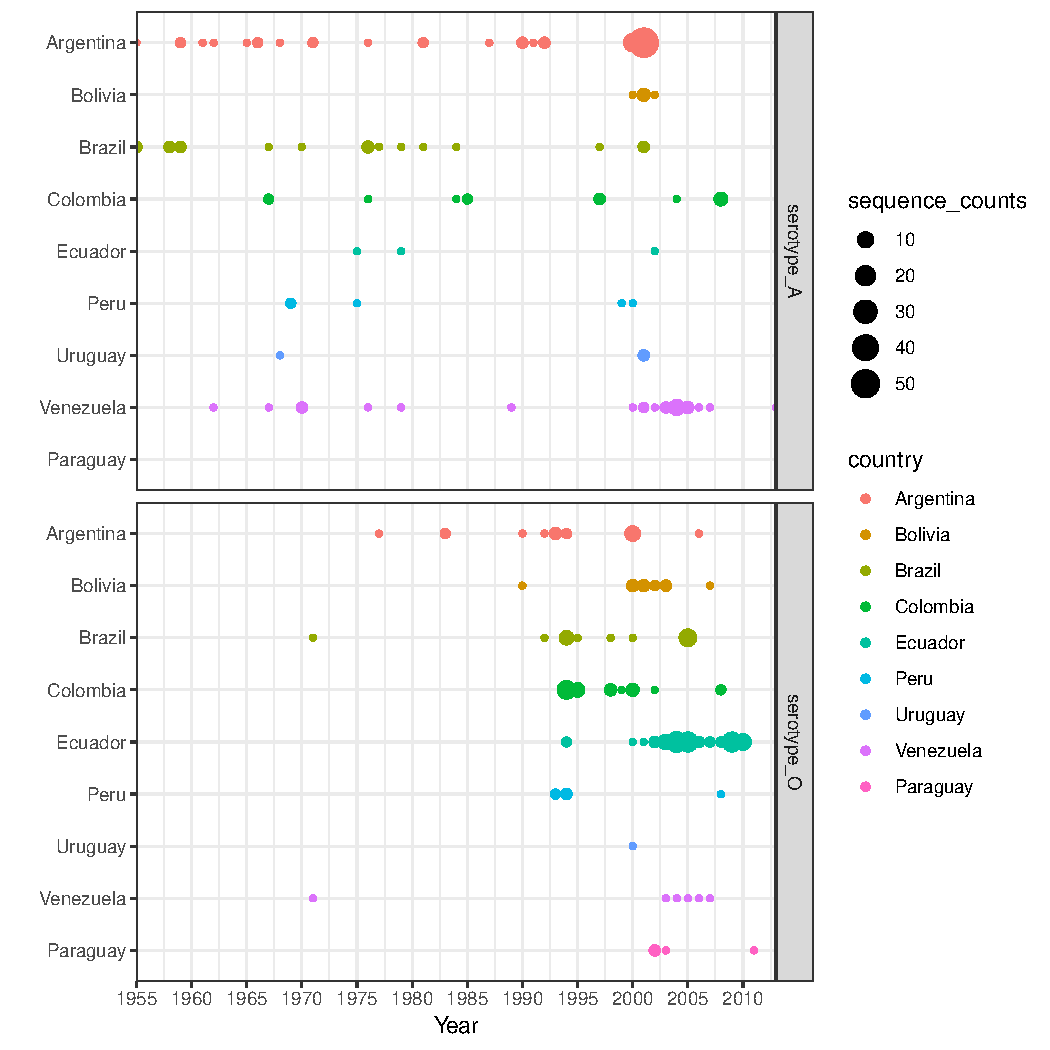
\includegraphics[scale=.80]{FIGURES/PLOTS/sampling_bubble_plot.pdf}
\end{center}
\caption{
\textbf{Spatio-temporal sampling pattern of the sequences used in this study.} Circle radius is proportional to number of sequences.
}
\label{sfig:sampling}
\end{figure}
\end{center}
% %%%%%%%%%%%%%%%%%%
% %%%%%%%%%%%%%%%%%%
\newpage
\begin{center}
\begin{figure}[H]
\begin{center}
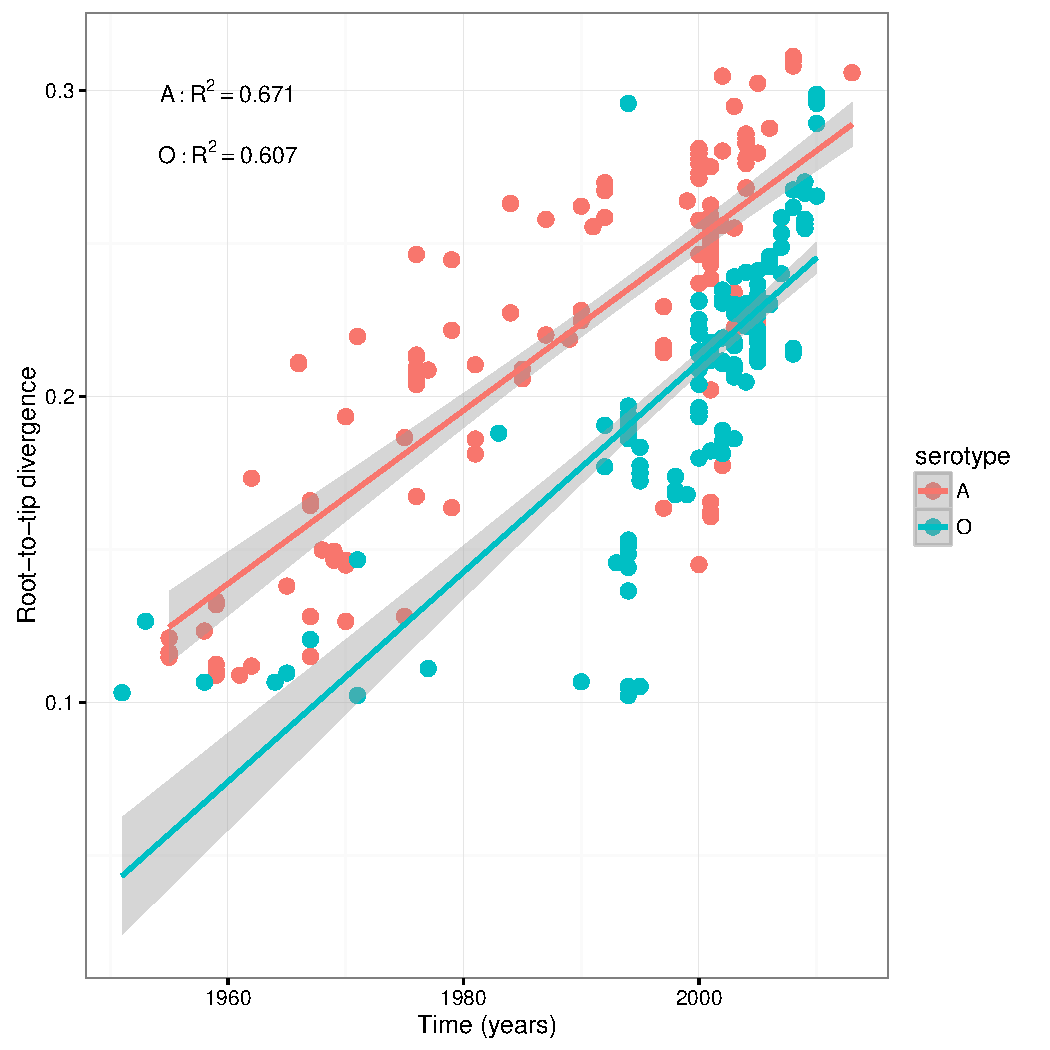
\includegraphics[scale=.75]{FIGURES/PLOTS/rdvs.pdf}
\end{center}
\caption{
\textbf{Root-to-tip divergence against sampling time for serotypes A and O.}
Maximum likelihood phylogenies were constructed with PhyML version 3.0~\citep{M-Guindon2003}. 
We root the trees such that the linear regression between the root-to-tip divergences and sampling times yields the smallest sum of squared residuals using the program TempEst~\citep{M-Rambaut2016}.
The linear trends, along with their 95\% prediction intervals (shaded) are shown.
}
\label{sfig:root-to-tip}
\end{figure}
\end{center}
% %%%%%%%%%%%%%%%%%%
% %%%%%%%%%%%%%%%%%%
\newpage
\begin{center}
\begin{figure}[H]
\begin{center}
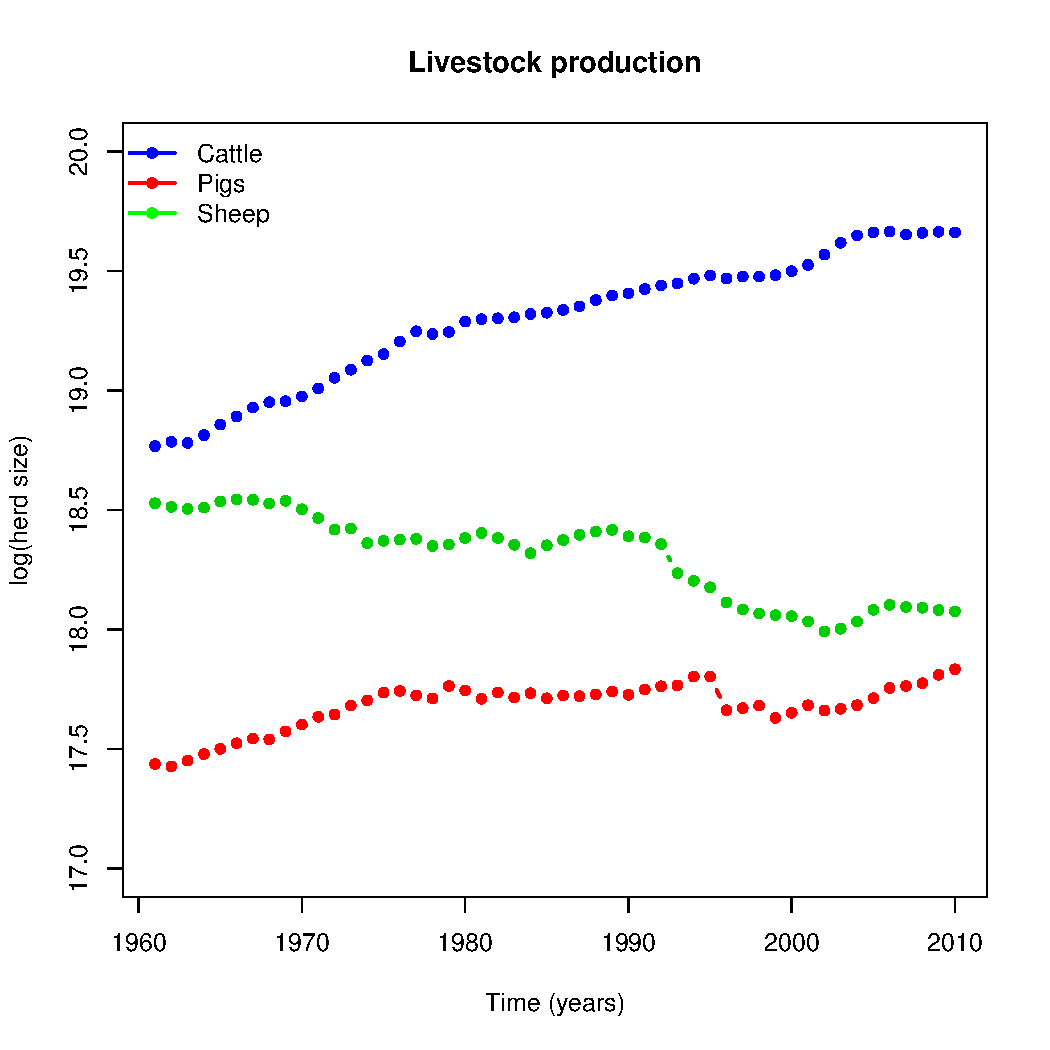
\includegraphics[scale=.80]{FIGURES/PLOTS/production.pdf}
\end{center}
\caption{
\textbf{Production time series for several livestock in South America.}
We show $\log$(\#~of heads) of live animals for pigs, sheep and cattle, goat and horses.
}
\label{sfig:prod}
\end{figure}
\end{center}
% %%%%%%%%%%%%%%%%%%%
% %%%%%%%%%%%%%%%%%%%
\newpage
\begin{center}
\begin{figure}[H]
\begin{center}
\subfigure[]{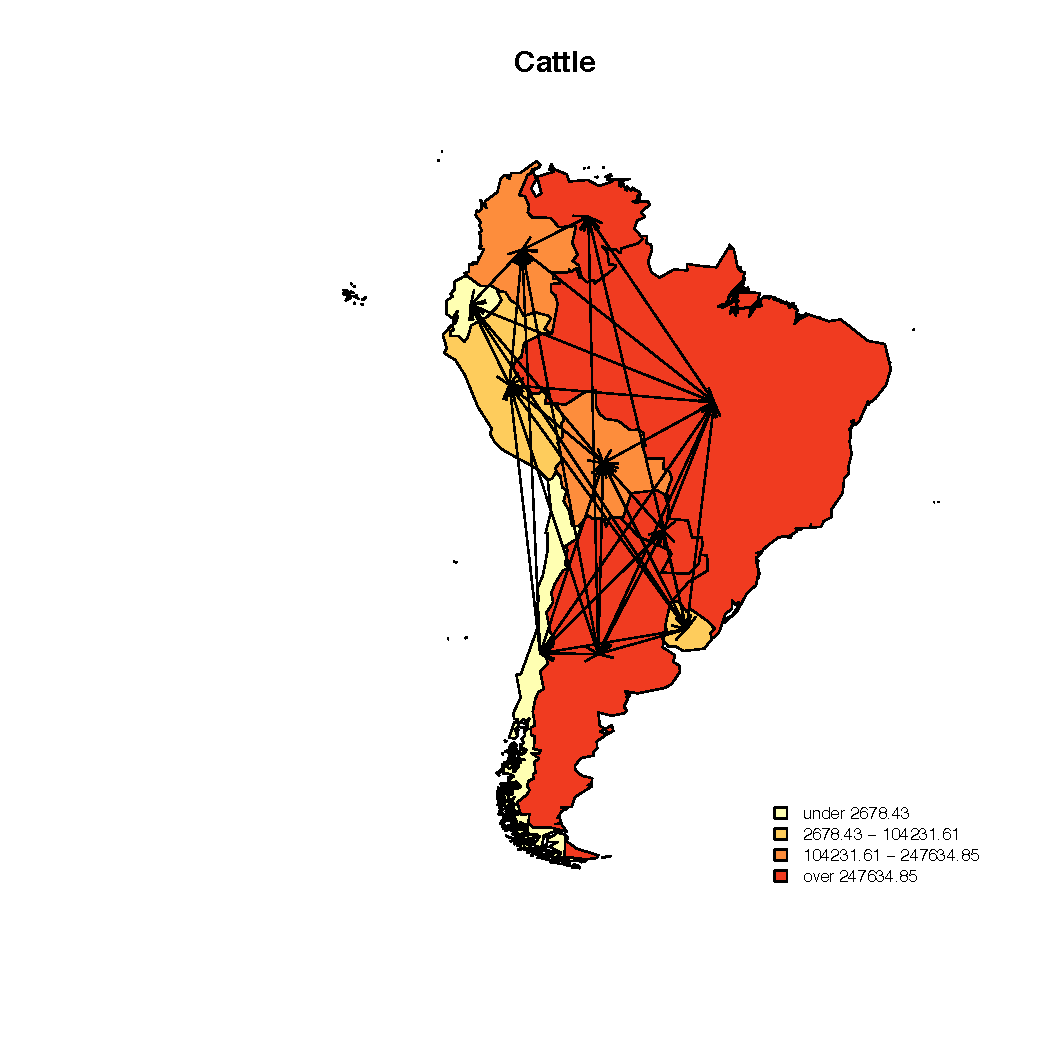
\includegraphics[scale=.600]{FIGURES/PLOTS/tradenets_cattle_s=0.pdf}}
\subfigure[]{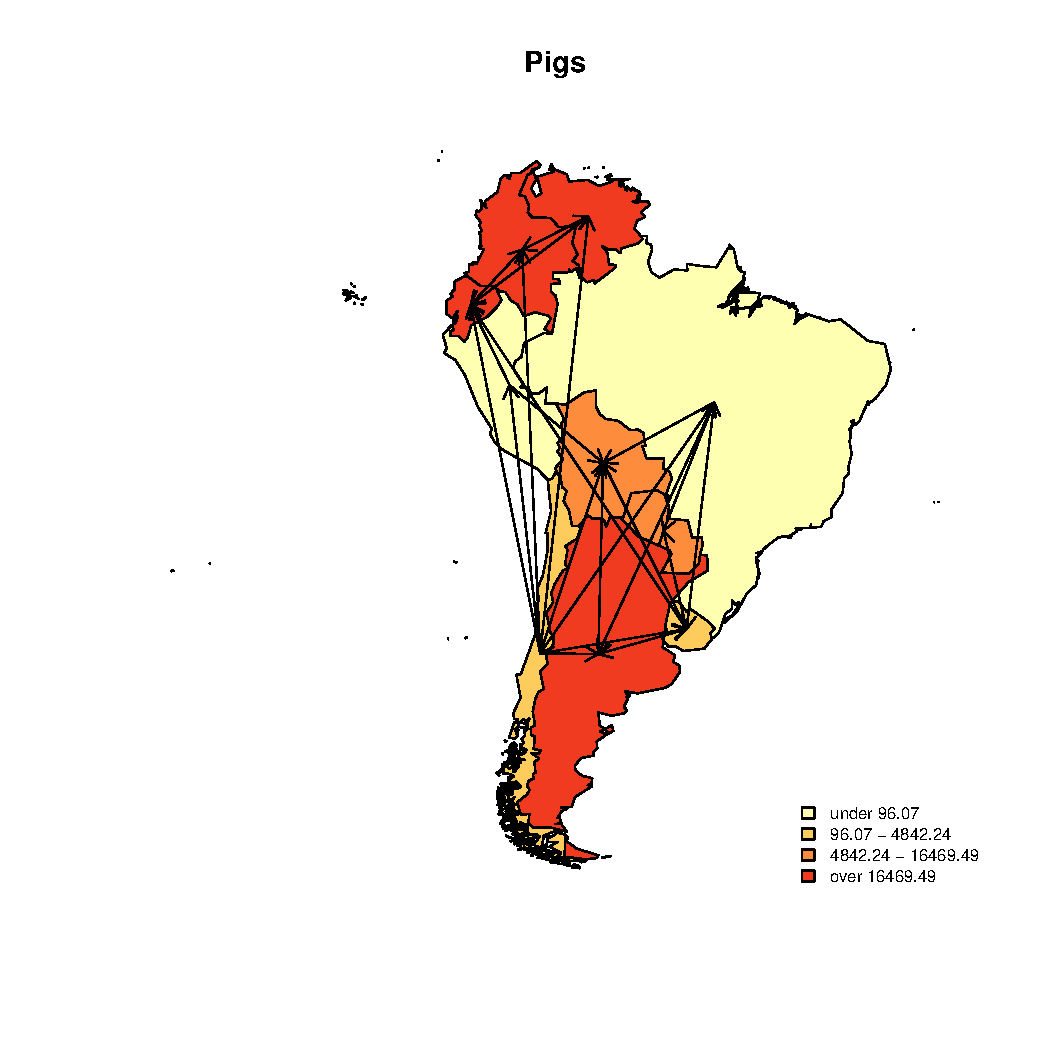
\includegraphics[scale=.600]{FIGURES/PLOTS/tradenets_pig_s=0.pdf}} \\
\subfigure[]{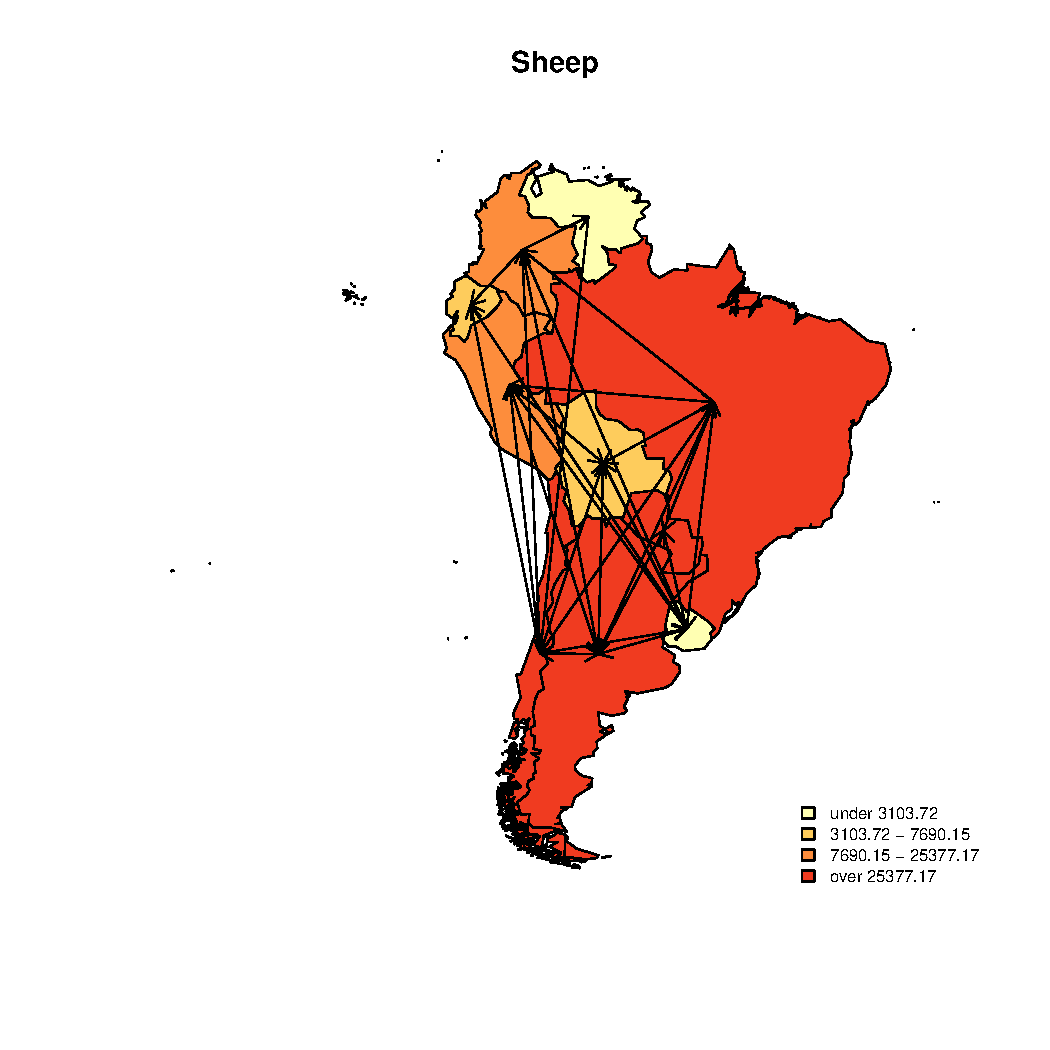
\includegraphics[scale=.600]{FIGURES/PLOTS/tradenets_sheep_s=0.pdf}}
\end{center}
\caption{
\textbf{Spatial networks of livestock trade in South America.}
We represent the total trade of live animals from $1986$ to $2017$.
Arrows connect countries if there was a non-zero number of exchanges between them.
Colour scale represents total exports in number of live animals.
In agreement with the data presented in Figure~\ref{sfig:prod}, the cattle network is the most connected, indicating that not only the number of animals has increased, but also the migration of this particular host is more frequent. 
Note the long range trade routes of sheep between Argentina and Colombia, which are absent from the pig network.
}
\label{sfig:tradenets}
\end{figure}
\end{center}
% %%%%%%%%%%%%%%%%%%%
% %%%%%%%%%%%%%%%%%%%
\newpage
\begin{center}
\begin{figure}[H]
\begin{center}
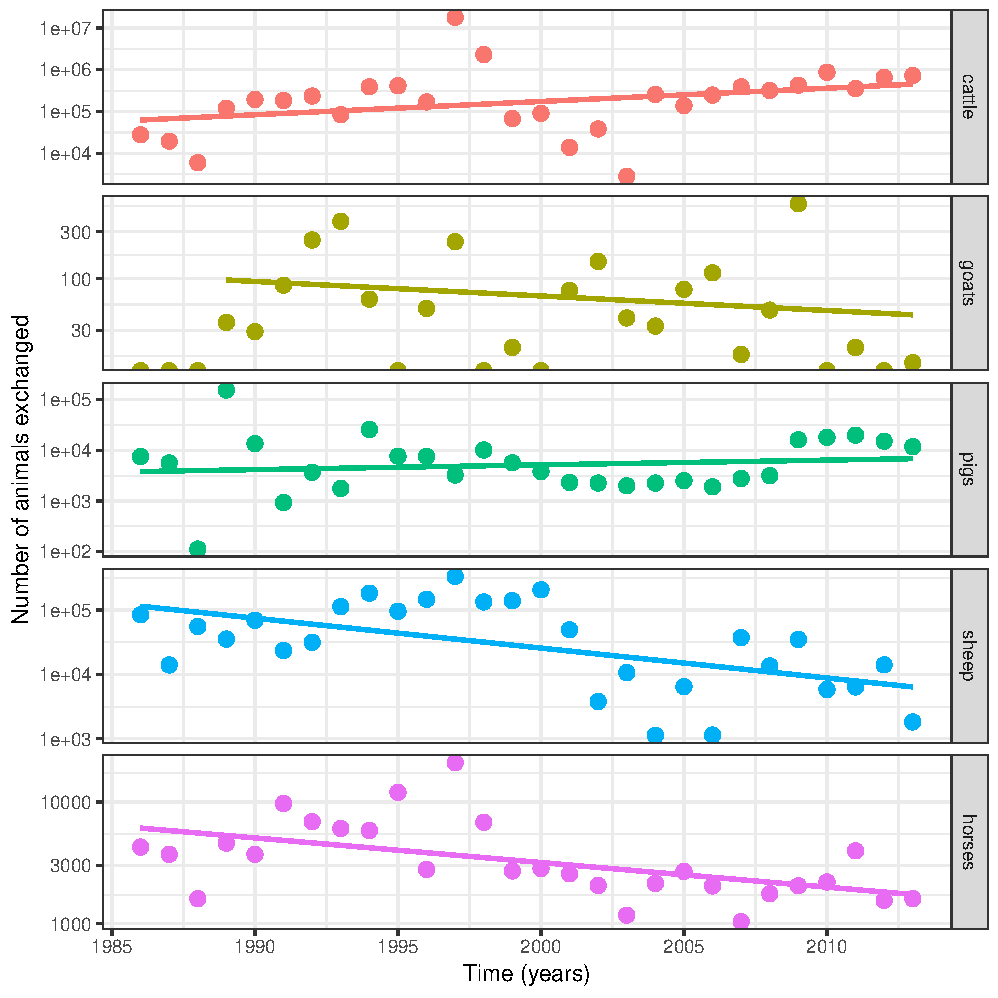
\includegraphics[scale=.80]{FIGURES/PLOTS/trade_through_time.pdf}
\end{center}
\caption{
\textbf{Overall livestock trade in South America through time.}
We show $\log$(\#~of heads) of live animals traded for pigs, sheep and cattle, goat and horses.
Solid lines are linear trends fitted using ordinary least squares.
}
\label{sfig:trade_temporal}
\end{figure}
\end{center}
% %%%%%%%%%%%%%%%%%%%
% %%%%%%%%%%%%%%%%%%%
\newpage
\begin{center}
\begin{figure}[H]
\begin{center}
\subfigure[]{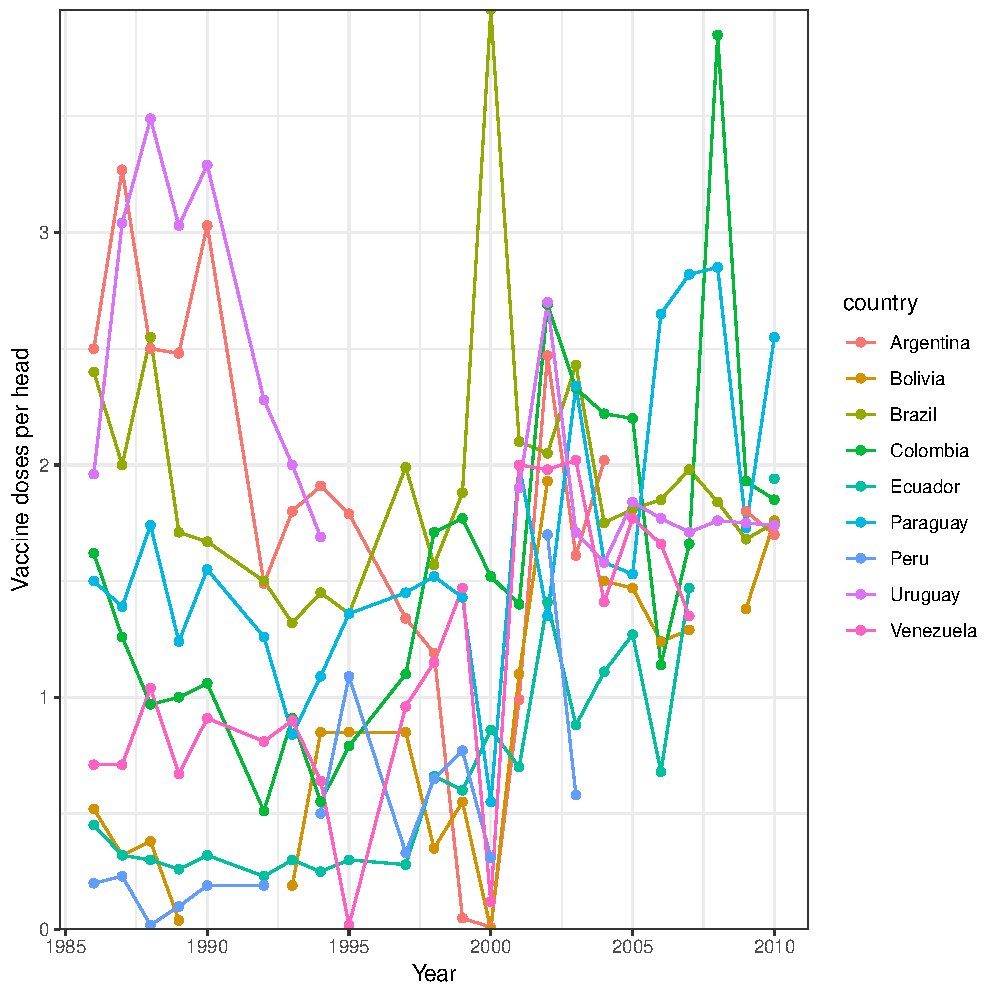
\includegraphics[scale=.600]{FIGURES/PLOTS/vaccination_per_country_time.pdf}} \\
\subfigure[]{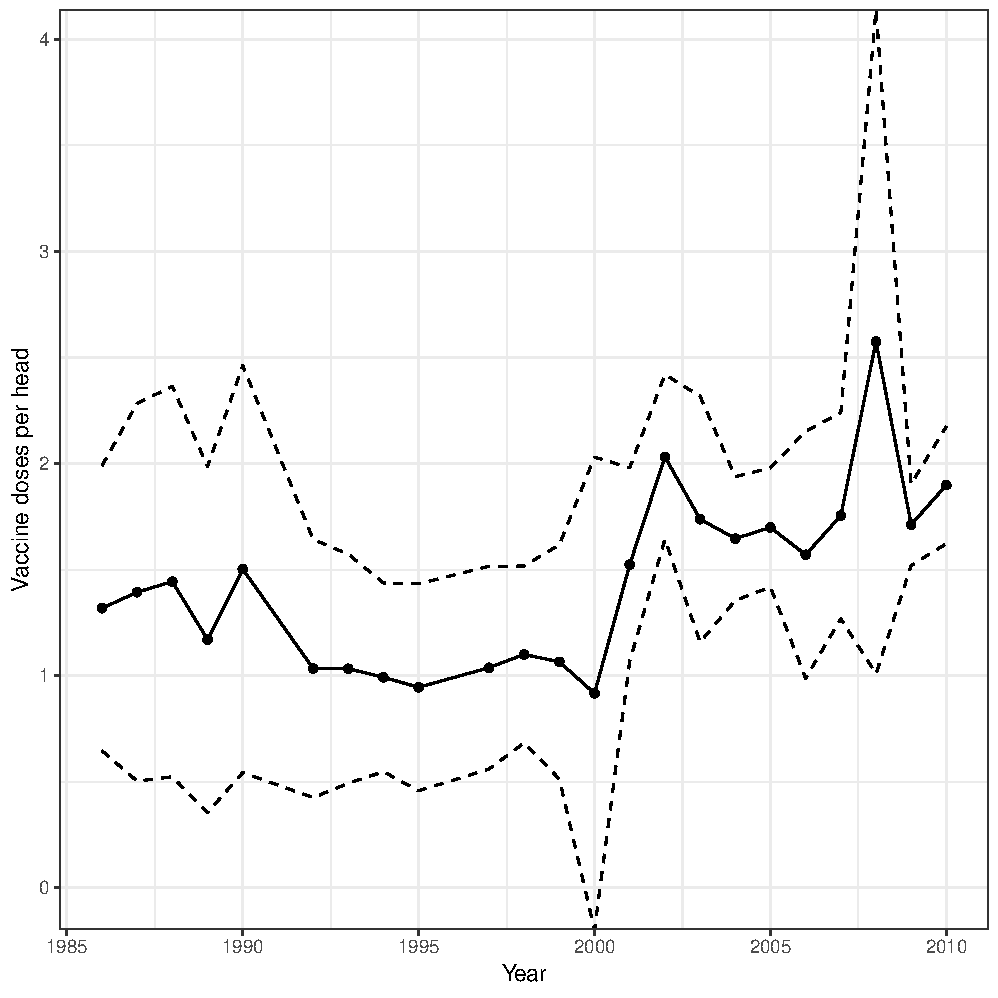
\includegraphics[scale=.600]{FIGURES/PLOTS/vaccination_overall_time.pdf}}
\end{center}
\caption{
\textbf{FMD vaccination in South America through time.}
We show the number of vaccine doses per cattle head per country (Panel a) and overall (Panel b).
In panel b the solid line shows the average and the dashed lines show Student t empirical intervals (see text).
}
\label{sfig:vaccination_temporal}
\end{figure}
\end{center}
% %%%%%%%%%%%%%%%%
% %%%%%%%%%%%%%%%%
% %%%%%%%%%%%%%%%%%%%
% %%%%%%%%%%%%%%%%%%%
\newpage
\begin{center}
\begin{figure}[H]
\begin{center}
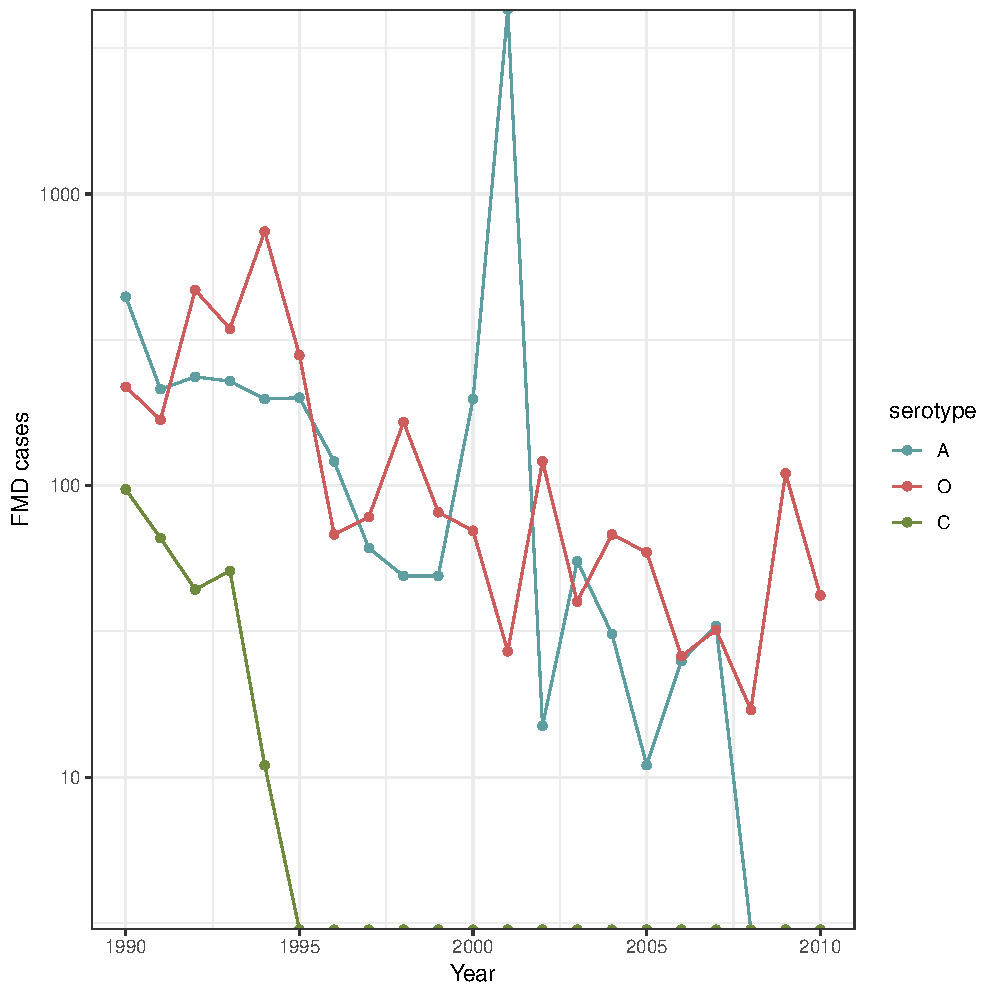
\includegraphics[scale=.600]{FIGURES/PLOTS/cases_per_serotype_per_time.pdf}
\end{center}
\caption{
\textbf{FMD cases per serotype in South America through time.}
We show the number of reported FMD cases per serotype.
}
\label{sfig:case_temporal}
\end{figure}
\end{center}
% %%%%%%%%%%%%%%%%
% %%%%%%%%%%%%%%%%
\newpage
\begin{center}
\begin{figure}[H]
\begin{center}
\subfigure[]{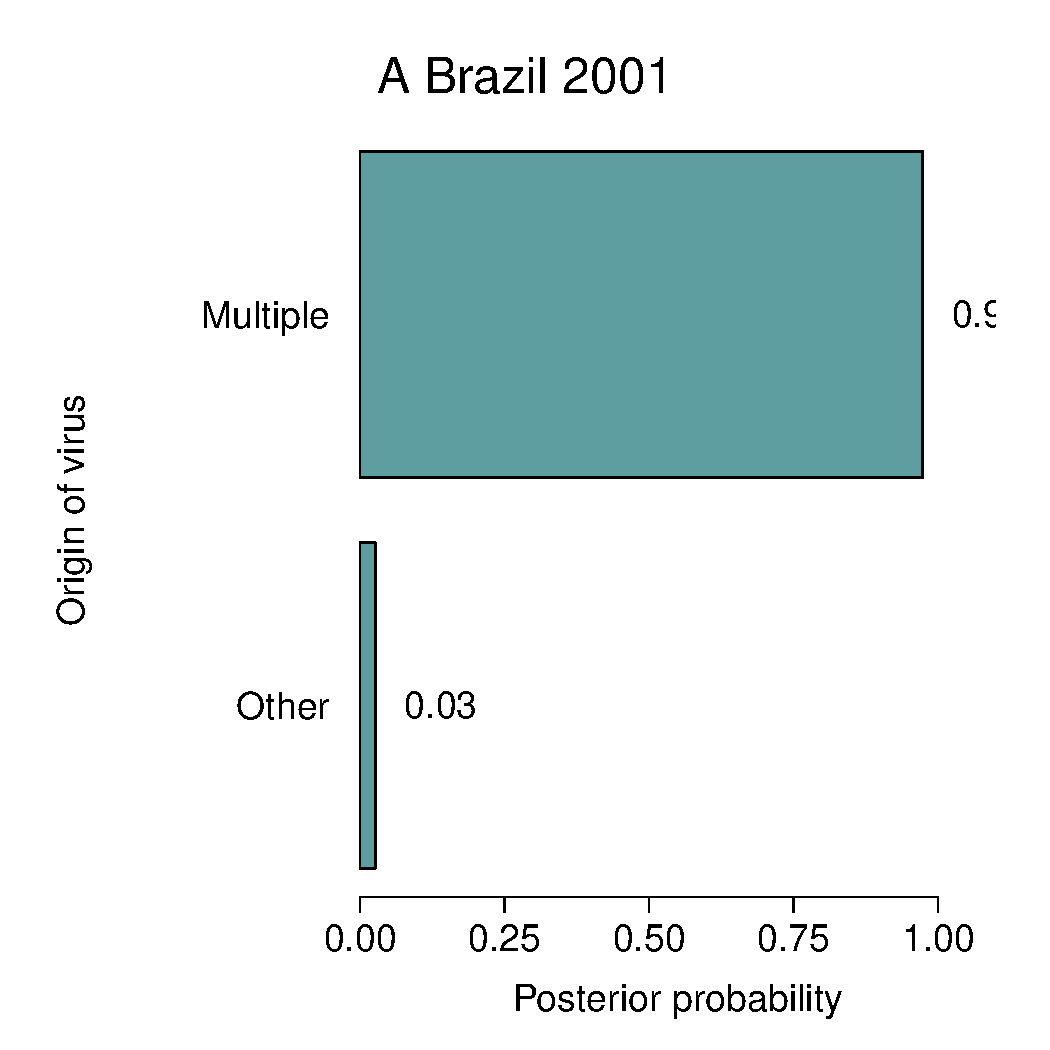
\includegraphics[scale=.35]{FIGURES/PLOTS/Origins_A_Brazil_2001.pdf}}
\subfigure[]{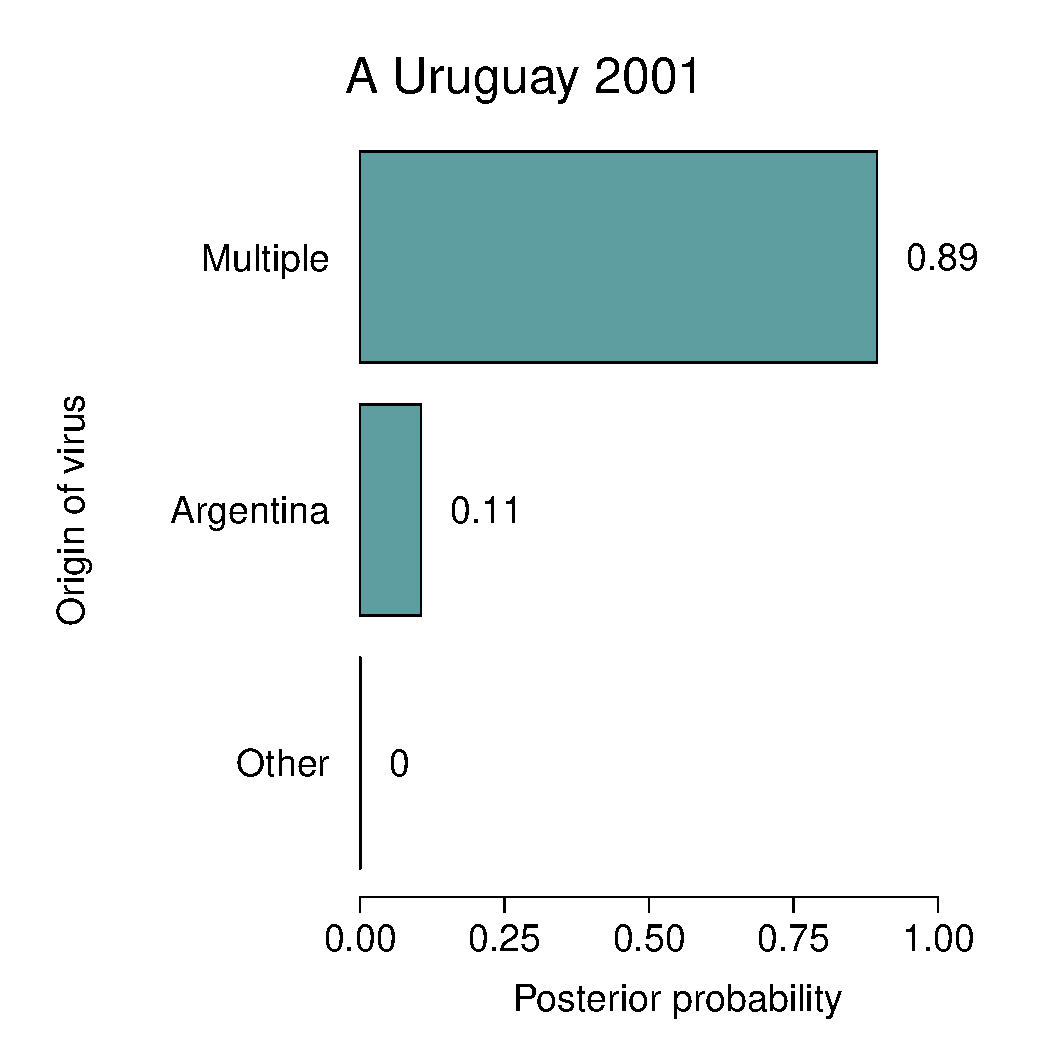
\includegraphics[scale=.35]{FIGURES/PLOTS/Origins_A_Uruguay_2001.pdf}}\\
\subfigure[]{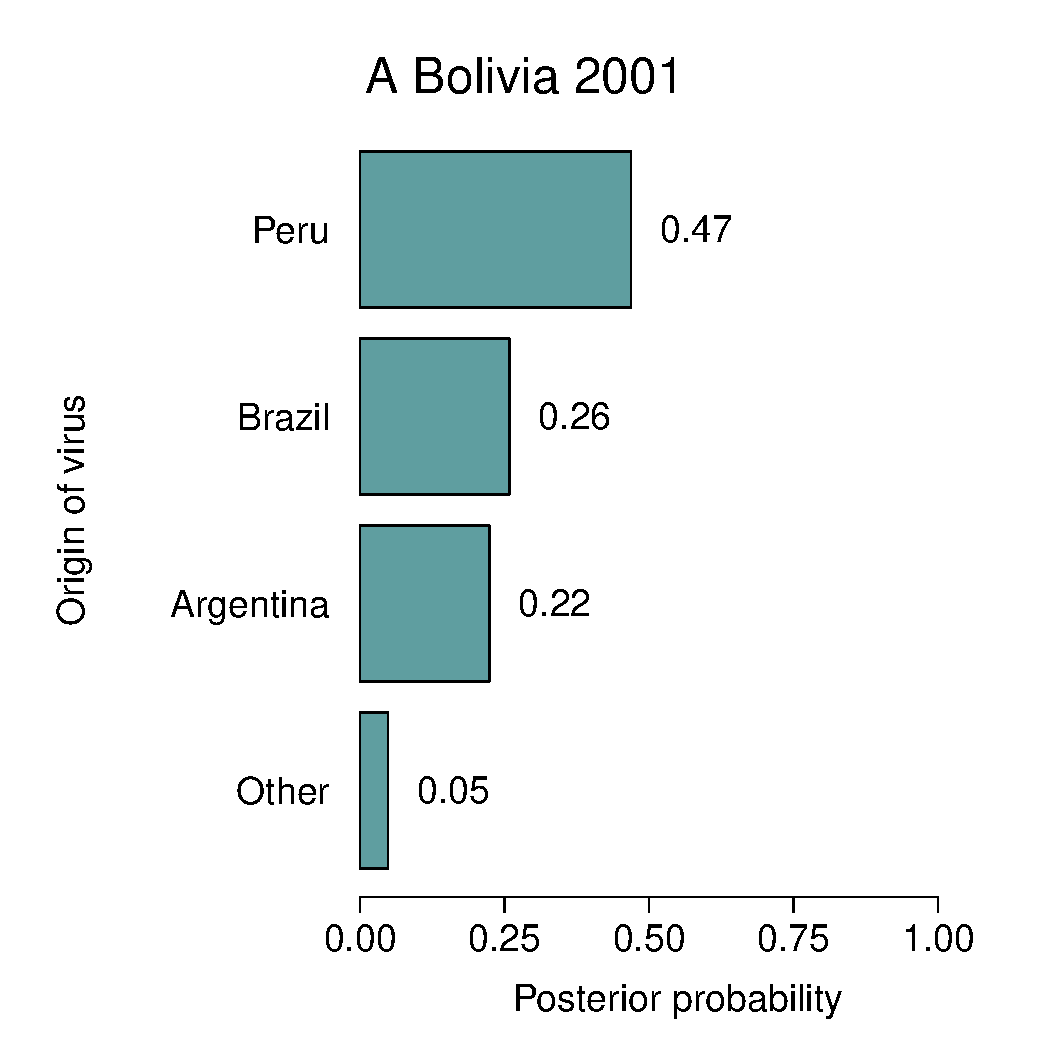
\includegraphics[scale=.35]{FIGURES/PLOTS/Origins_A_Bolivia_2001.pdf}}
\subfigure[]{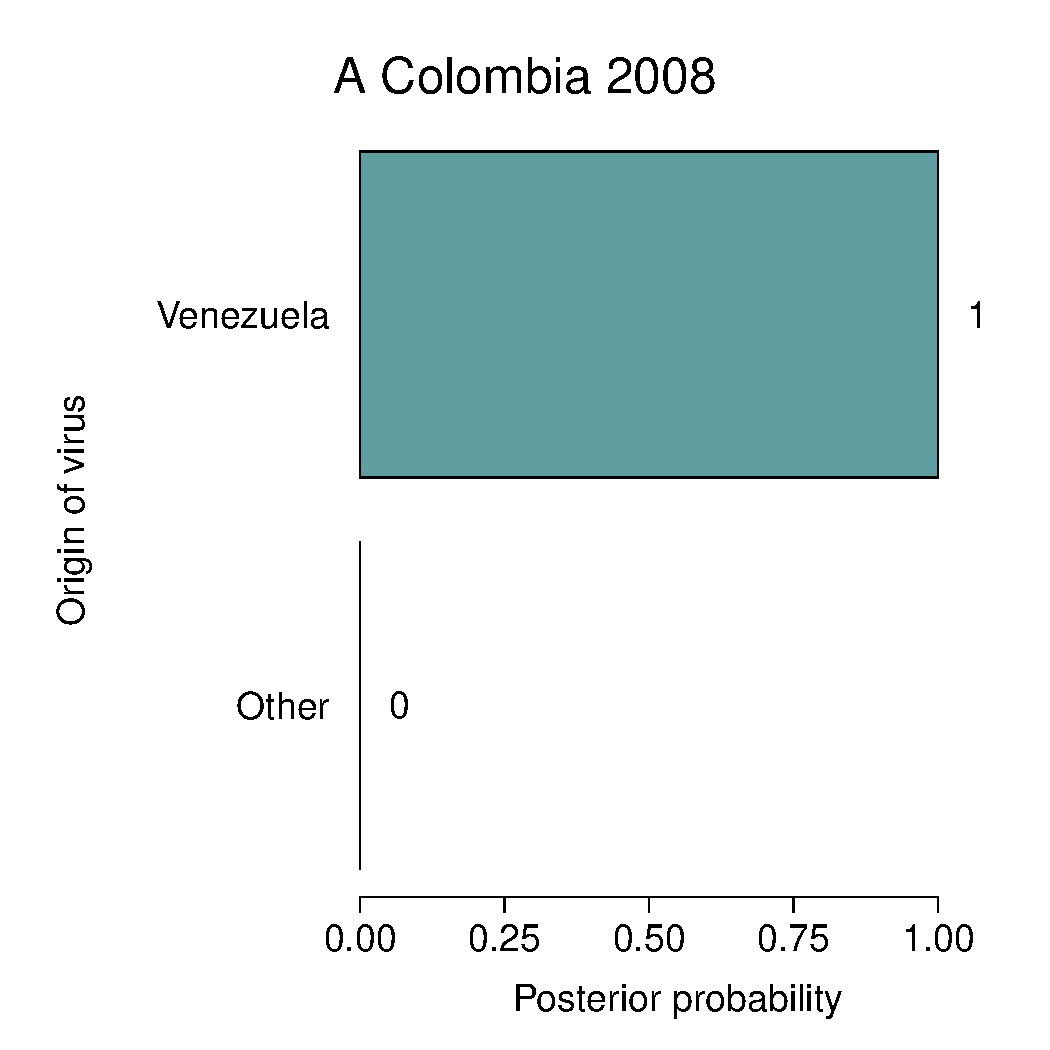
\includegraphics[scale=.35]{FIGURES/PLOTS/Origins_A_Colombia_2008.pdf}}\\
\subfigure[]{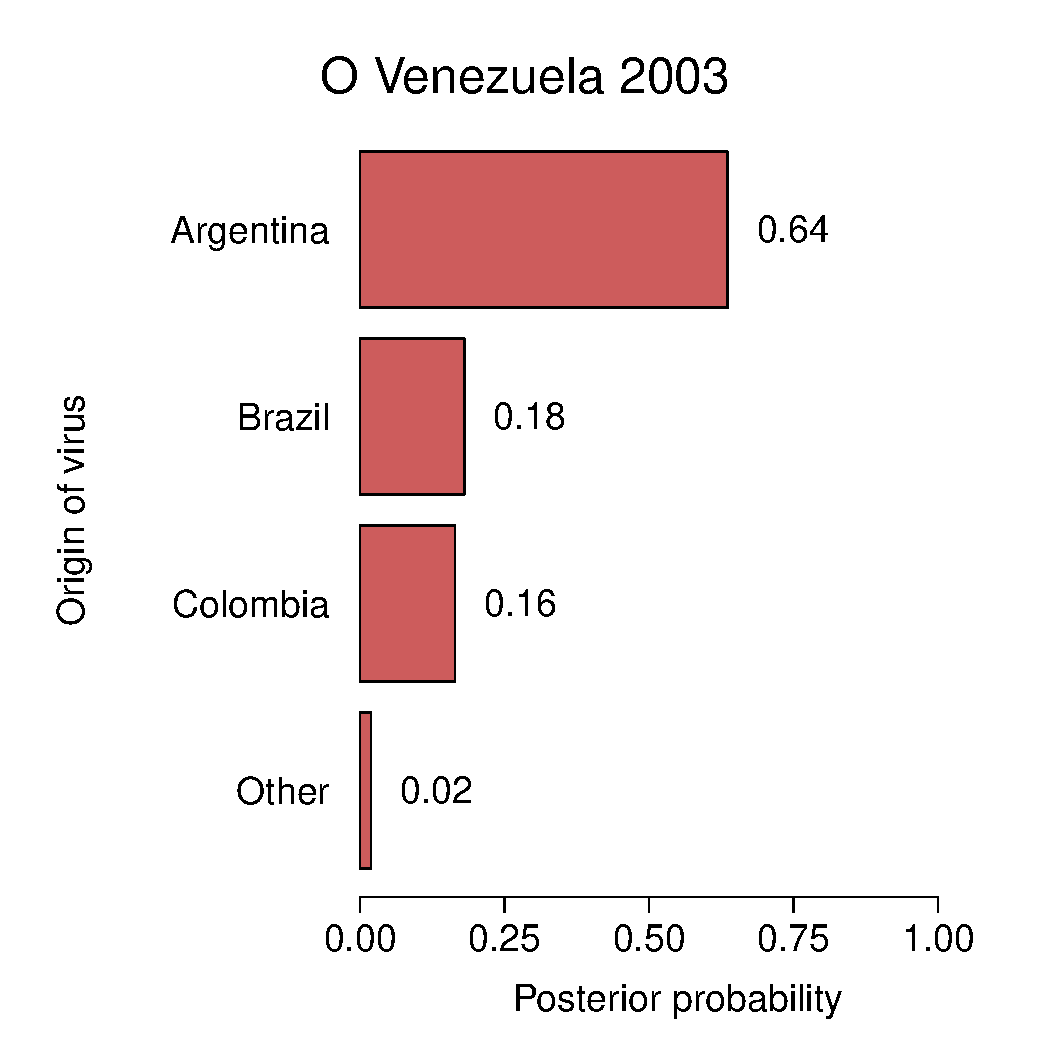
\includegraphics[scale=.35]{FIGURES/PLOTS/Origins_O_Venezuela_2003.pdf}}
\subfigure[]{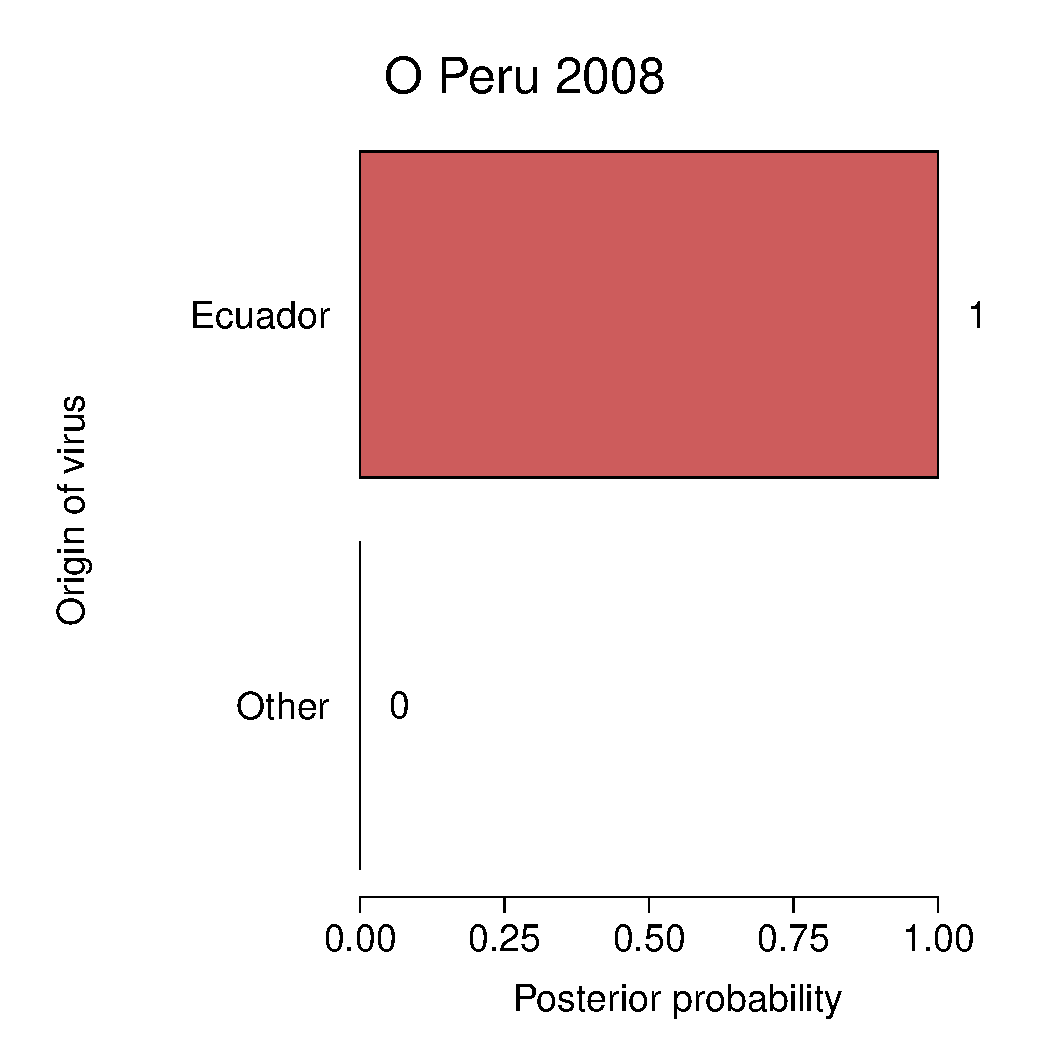
\includegraphics[scale=.35]{FIGURES/PLOTS/Origins_O_Peru_2008.pdf}}
\end{center}
\caption{\textbf{Epidemic tracing of FMDV in South America -- extra results}.
For serotype A, we show the most probable origins of the 2001 outbreaks in Brazil (A), Uruguay (B) and Bolivia (C), along with the origins of the Colombian 2008 strain (D).
Panels E and F show the origins of serotype O in Venezuela 2003 and Peru 2008, respectively.
}
\label{sfig:epitrac}
\end{figure}
\end{center}
% %%%%%%%%%%%%%%%%
% %%%%%%%%%%%%%%%%
\newpage
\begin{center}
\begin{figure}[H]
\begin{center}
\subfigure[Constant size, empirical dates]{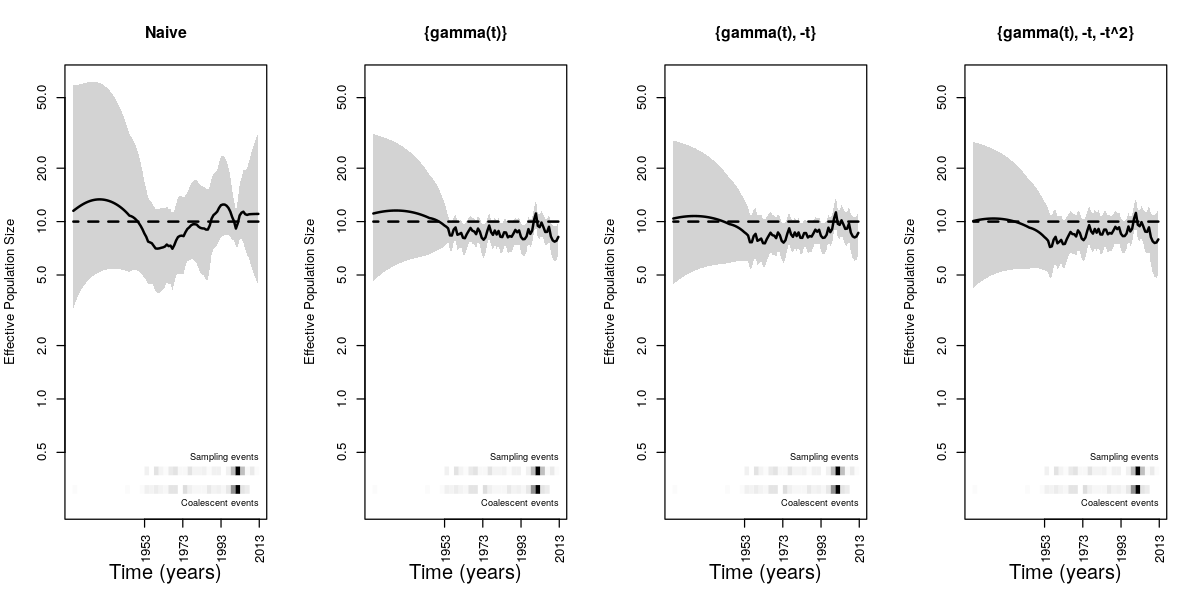
\includegraphics[scale=.38]{FIGURES/PLOTS/typical_reconstruction_scenario_A_serotype_A.png}}\\
\subfigure[Exponential growth, empirical dates]{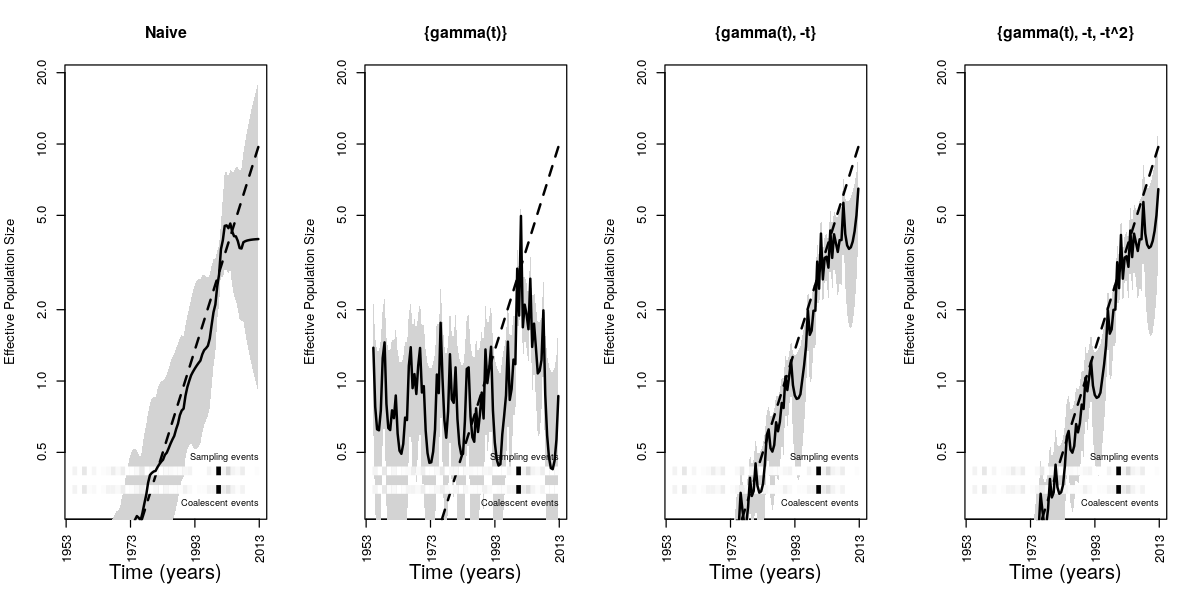
\includegraphics[scale=.38]{FIGURES/PLOTS/typical_reconstruction_scenario_B_serotype_A.png}}\\
\subfigure[Constant size, uniform dates]{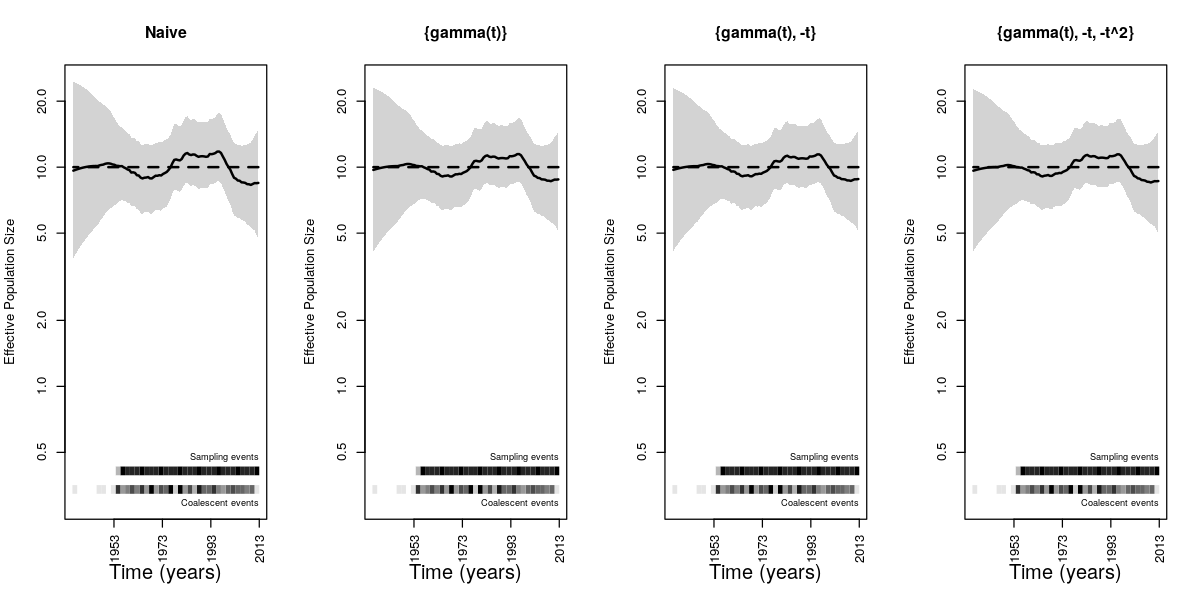
\includegraphics[scale=.38]{FIGURES/PLOTS/typical_reconstruction_scenario_C_serotype_A.png}}\\
\subfigure[Exponential size, uniform dates]{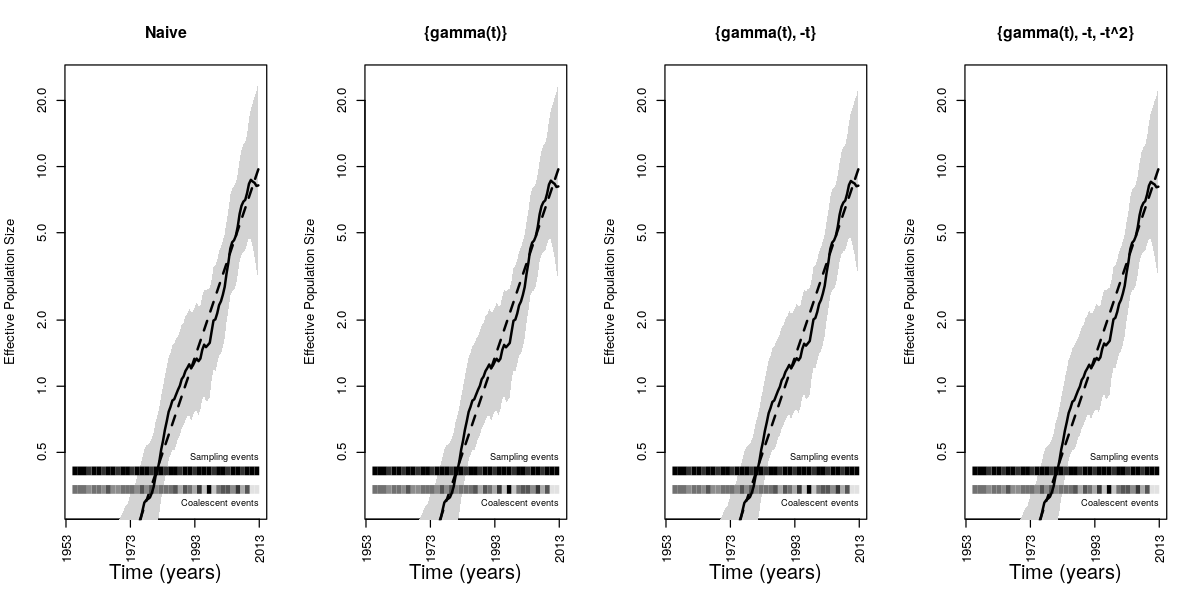
\includegraphics[scale=.38]{FIGURES/PLOTS/typical_reconstruction_scenario_D_serotype_A.png}}\\
\end{center}
\caption{\textbf{Typical reconstructions in BNPR simulation study, serotype A}.
A: constant population size $N_e = 10$ with empirical dates; B: exponential population growth with $N_0 = 10$ and $r = 0.1$ with empirical dates; C: constant population size $N_e = 10$ with uniform temporal sampling; D: exponential population growth with $N_0 = 10$ and $r = 0.1$ with uniform temporal sampling.
Dashed line shows the true population trajectory, and shaded are shows the 95\% BCI.
Vertical tiles show the four models considered (see text for details).
}
\label{sfig:reconplots_A}
\end{figure}
\end{center}
% %%%%%%%%%%%%%%%%
% %%%%%%%%%%%%%%%%
\newpage
\begin{center}
\begin{figure}[H]
\begin{center}
\subfigure[Constant size, empirical date]{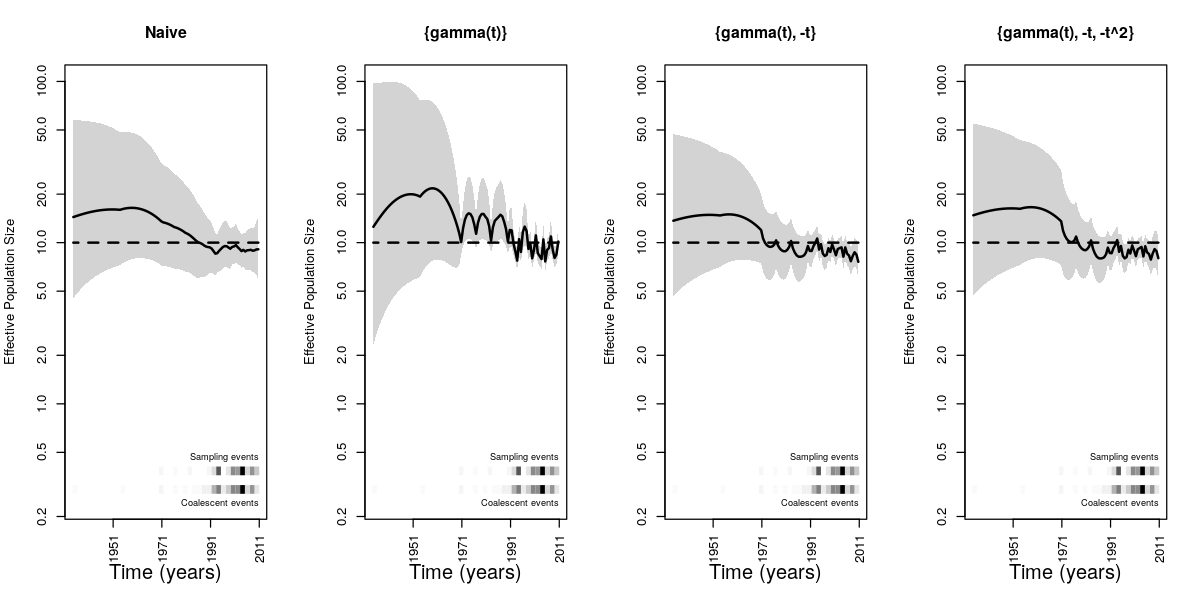
\includegraphics[scale=.38]{FIGURES/PLOTS/typical_reconstruction_scenario_A_serotype_O.png}}\\
\subfigure[Exponential growth, empirical dates]{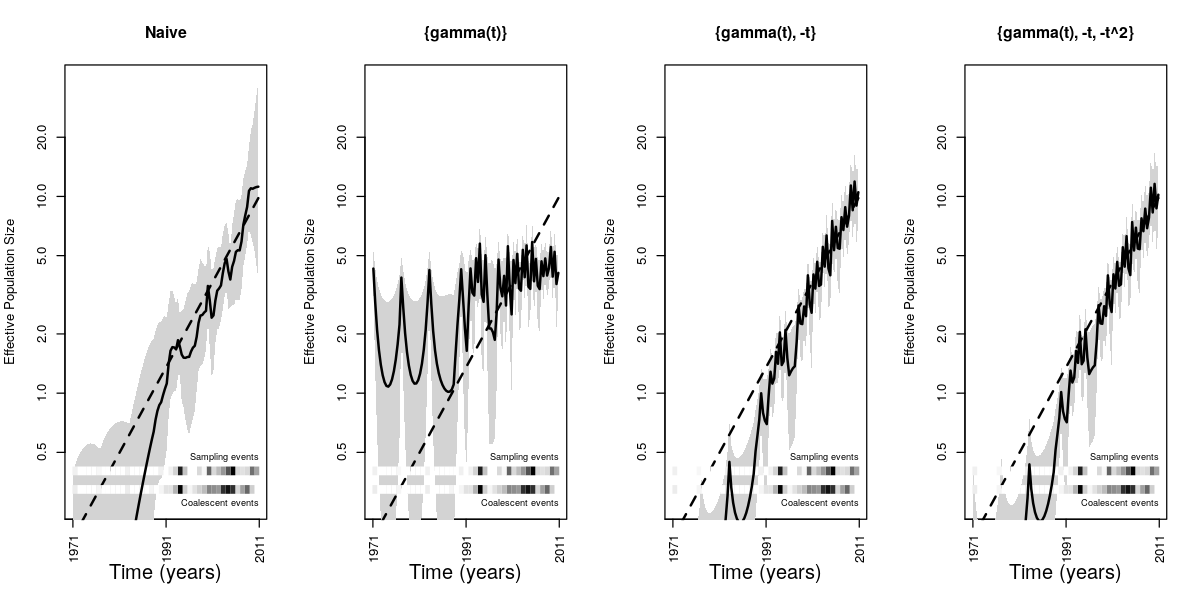
\includegraphics[scale=.38]{FIGURES/PLOTS/typical_reconstruction_scenario_B_serotype_O.png}}\\
\subfigure[Constant size, uniform dates]{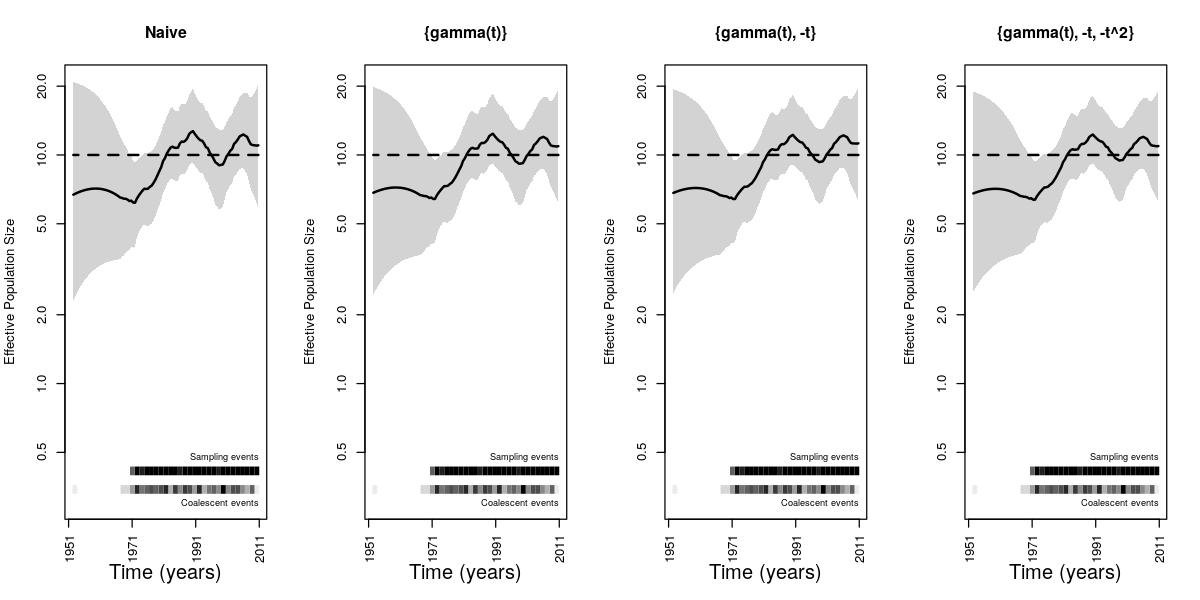
\includegraphics[scale=.38]{FIGURES/PLOTS/typical_reconstruction_scenario_C_serotype_O.png}}\\
\subfigure[Exponential size, uniform dates]{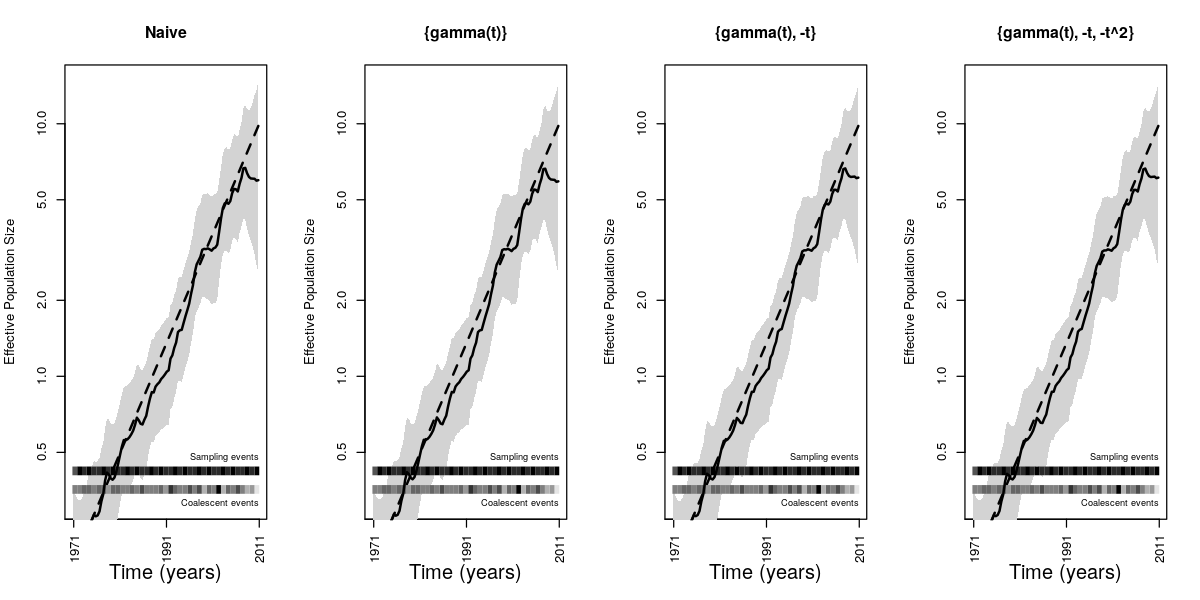
\includegraphics[scale=.38]{FIGURES/PLOTS/typical_reconstruction_scenario_D_serotype_O.png}}\\
\end{center}
\caption{\textbf{Typical reconstructions in BNPR simulation study, serotype O}.
A: constant population size $N_e = 10$ with empirical dates; B: exponential population growth with $N_0 = 10$ and $r = 0.1$ with empirical dates; C: constant population size $N_e = 10$ with uniform temporal sampling; D: exponential population growth with $N_0 = 10$ and $r = 0.1$ with uniform temporal sampling.
Dashed line shows the true population trajectory, and shaded are shows the 95\% BCI.
Vertical tiles show the four models considered (see text for details).
}
\label{sfig:reconplots_O}
\end{figure}
\end{center}
% %%%%%%%%%%%%%%%%
% %%%%%%%%%%%%%%%%
\newpage
\begin{center}
\begin{figure}[H]
\begin{center}
\subfigure[Constant size, empirical date]{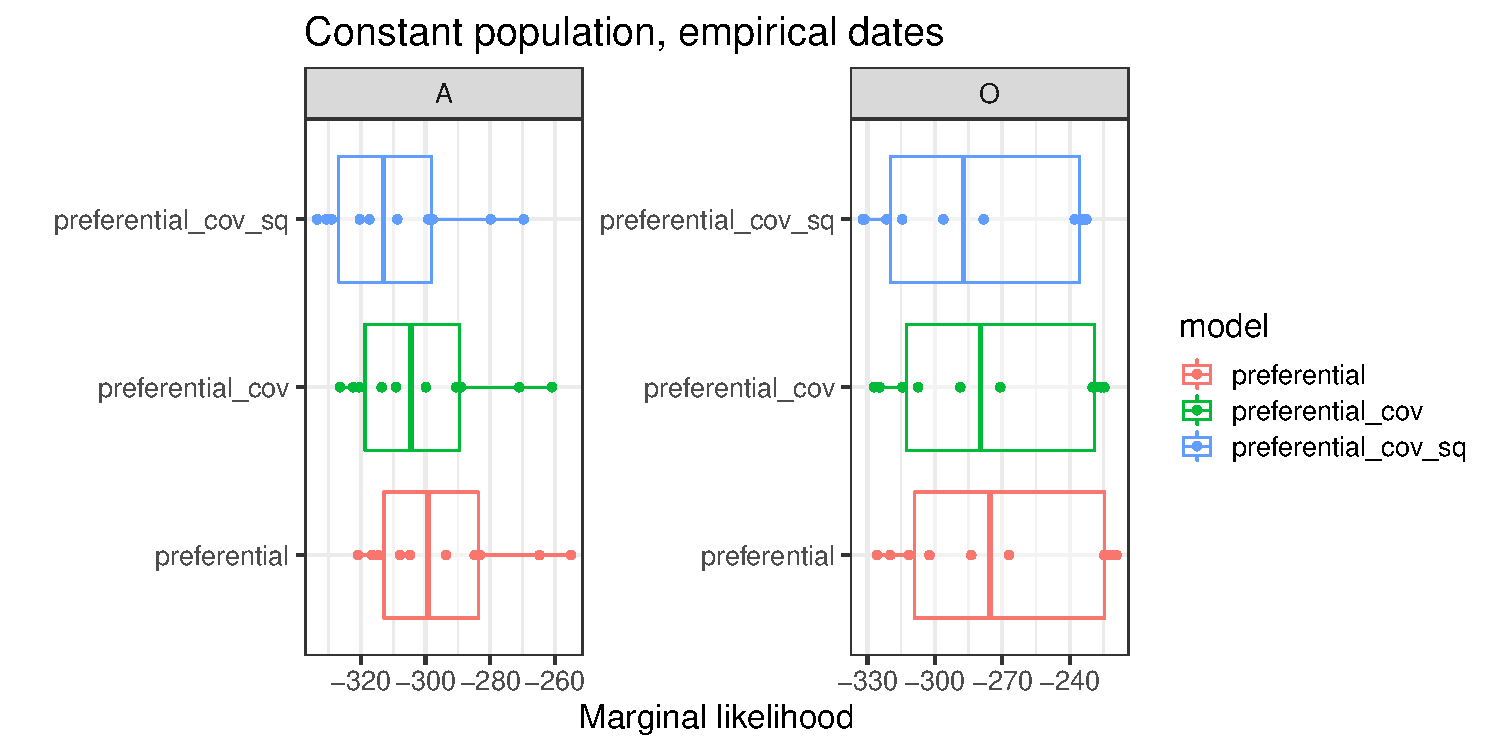
\includegraphics[scale=.3]{FIGURES/PLOTS/BNPR_simulations_scenario_A.pdf}}
\subfigure[Exponential growth, empirical dates]{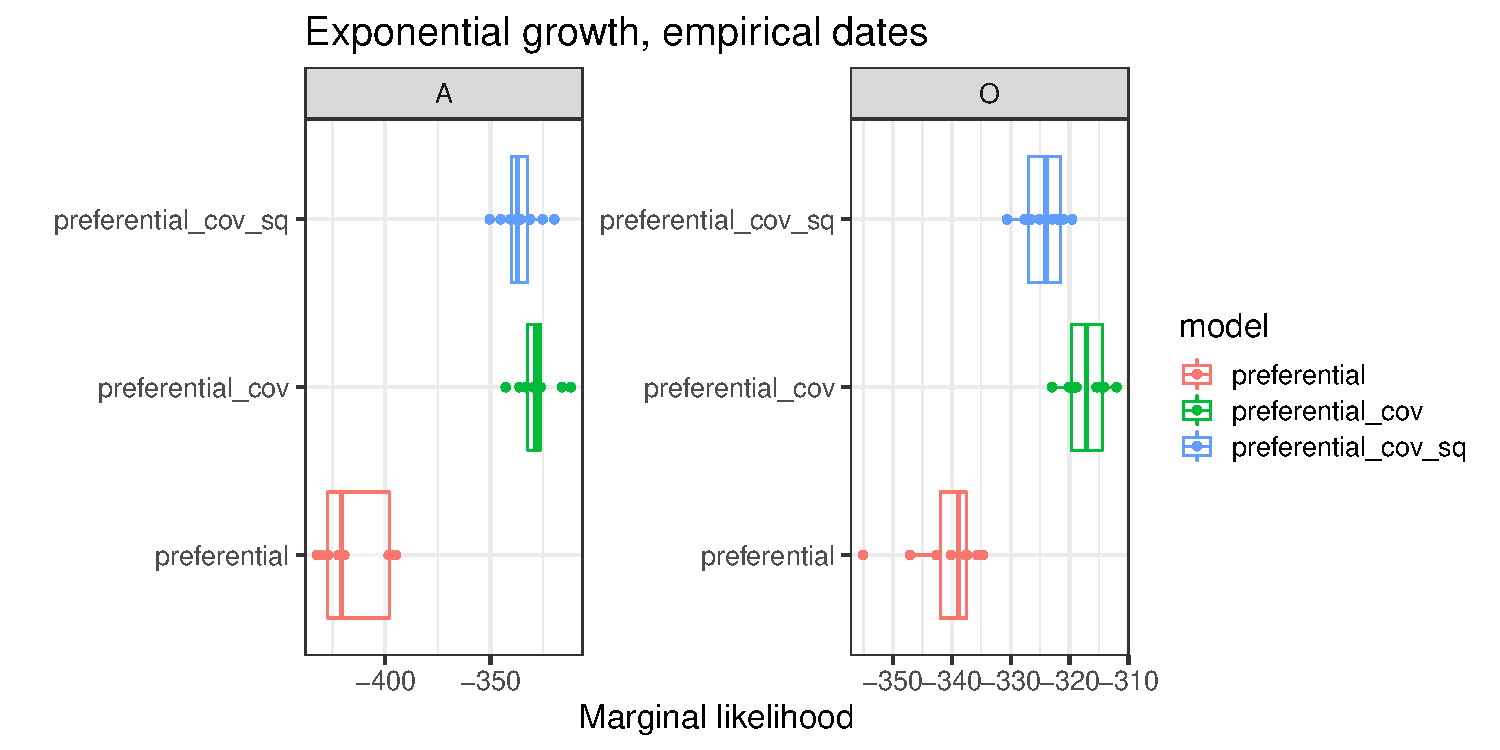
\includegraphics[scale=.3]{FIGURES/PLOTS/BNPR_simulations_scenario_B.pdf}}\\
\subfigure[Constant size, uniform dates]{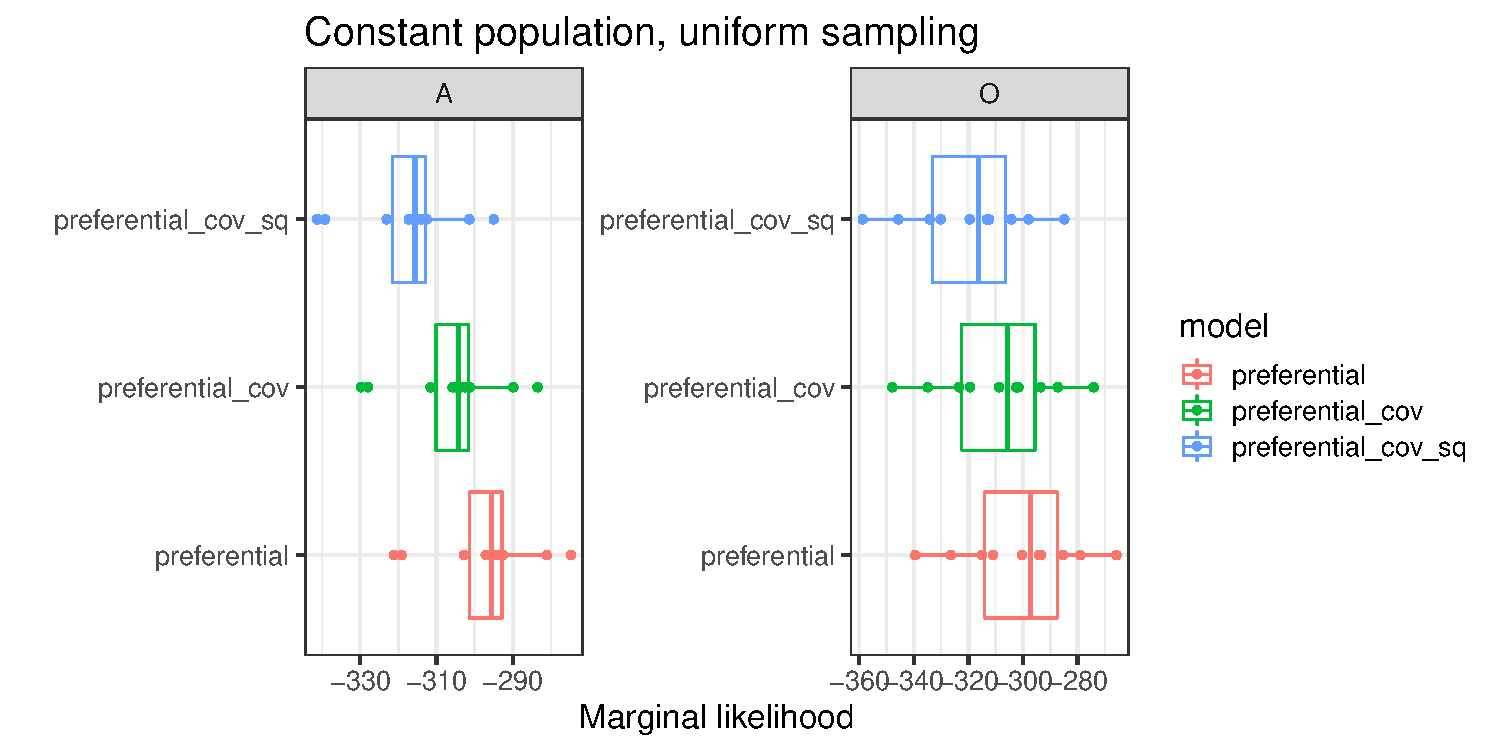
\includegraphics[scale=.3]{FIGURES/PLOTS/BNPR_simulations_scenario_C.pdf}}
\subfigure[Exponential size, uniform dates]{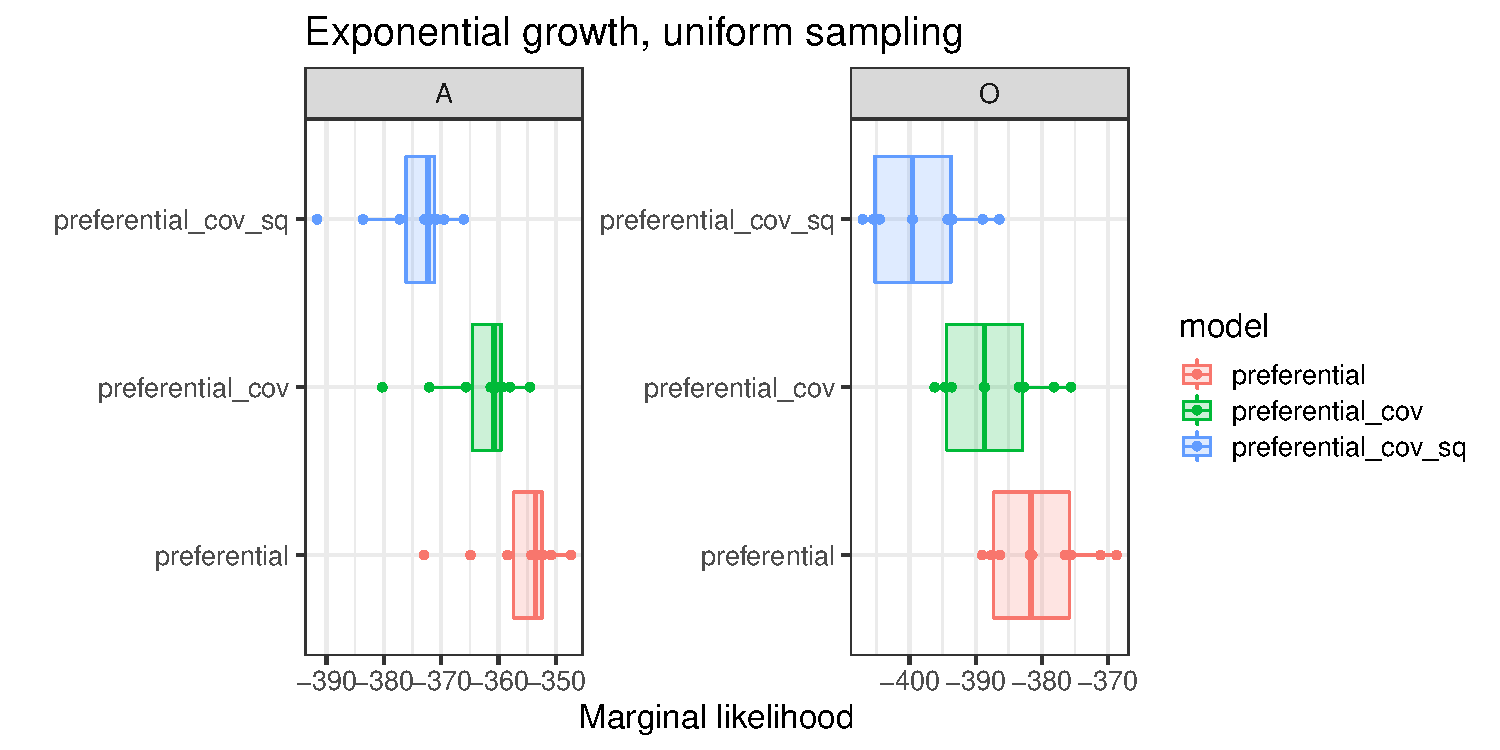
\includegraphics[scale=.3]{FIGURES/PLOTS/BNPR_simulations_scenario_D.pdf}}
\end{center}
\caption{\textbf{Estimated (log) marginal likelihoods for the BNPR simulation study}.
A: constant population size $N_e = 10$ with empirical dates; B: exponential population growth with $N_0 = 10$ and $r = 0.1$ with empirical dates; C: constant population size $N_e = 10$ with uniform temporal sampling; D: exponential population growth with $N_0 = 10$ and $r = 0.1$ with uniform temporal sampling.
Points show actual data points and boxplots show the quantiles.
Only results for models 1, 2 and 3 are shown because model 0 is not directly comparable (see text).
}
\label{sfig:BNPR_simu_marglikes}
\end{figure}
\end{center}
% %%%%%%%%%%%%%%%%
% %%%%%%%%%%%%%%%%
\newpage
\begin{center}
\begin{figure}[H]
\begin{center}
\subfigure[Serotype A]{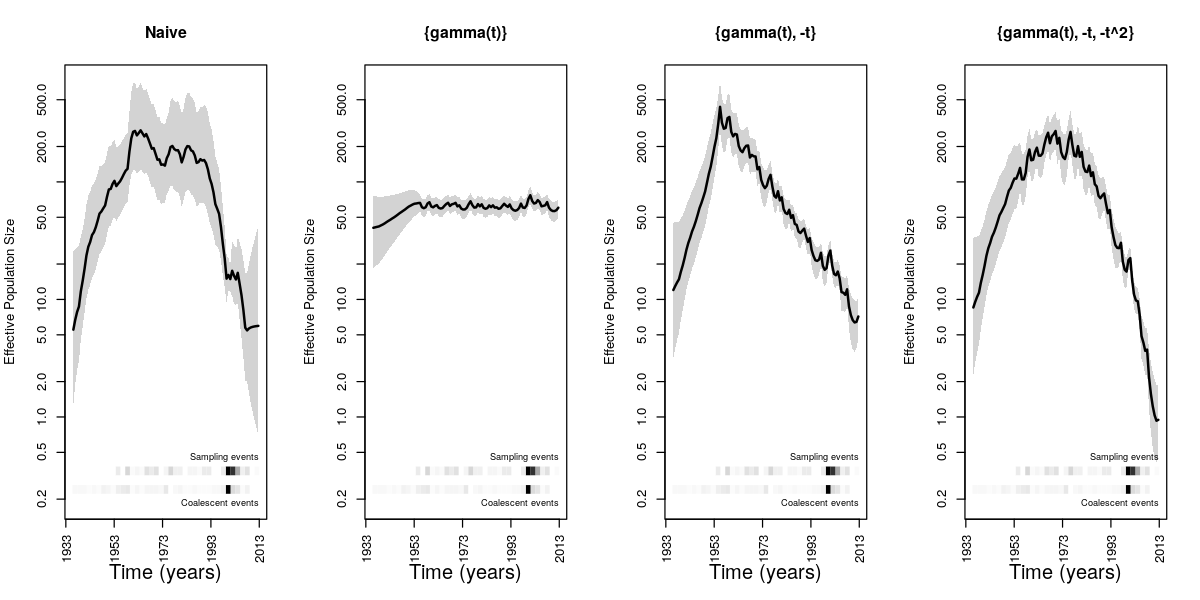
\includegraphics[scale=.600]{FIGURES/PLOTS/typical_reconstruction_BNPR_serotype_A.png}} \\
\subfigure[Serotype O]{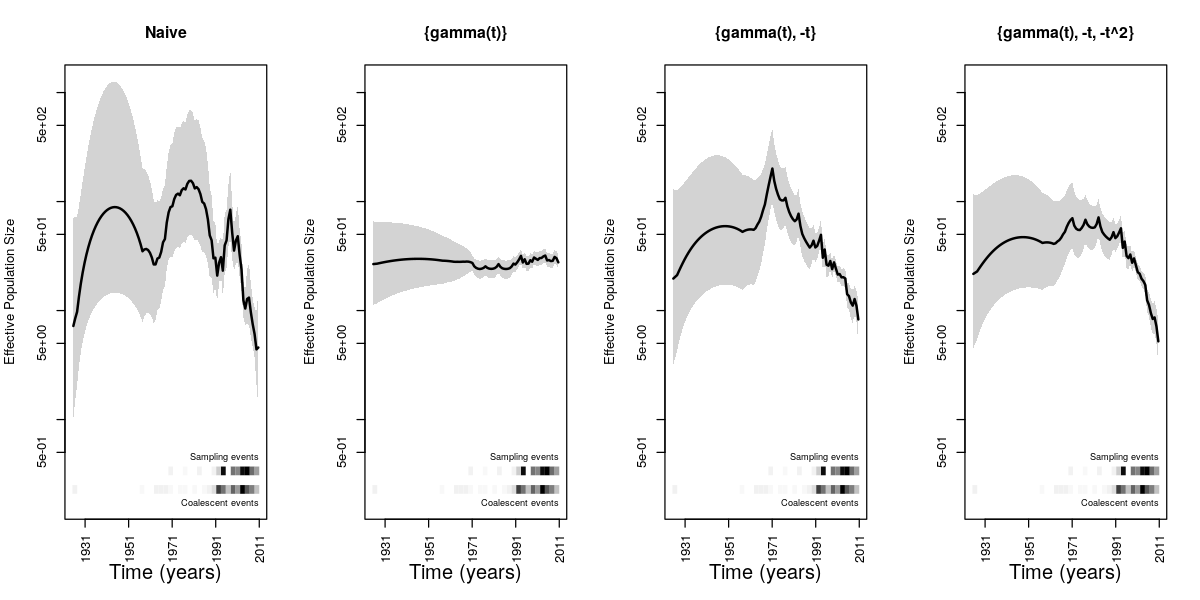
\includegraphics[scale=.600]{FIGURES/PLOTS/typical_reconstruction_BNPR_serotype_O.png}}
\end{center}
\caption{
\textbf{Population reconstructions for serotypes A and O under different preferential sampling models.}
Reconstructions for serotype A are shown in panel A, while reconstructions for serotype O are in panel B.
}
\label{sfig:full_reconstructions_BNPR}
\end{figure}
\end{center}
% %%%%%%%%%%%%%%%%
% %%%%%%%%%%%%%%%%
%%%%%%%%%%%%%%%%%%%%%%%%%%%%%%%%%%%%%%%%%%%%%%%%%%%%%%%%%%%%%%%%%%%%%%%%%%%%%%%%%%%
%%%%%%%%%%%%%%%%%%%%%%%%%%%%%%%%%%%%%%%%%%%%%%%%%%%%%%%%%%%%%%%%%%%%%%%%%%%%%%%%%%%
\newpage
\begin{center}
 \begin{longtable}{ccc}
  \caption{\textbf{Accession numbers, date and country of collection for the serotype A sequences}. When only the year of collection was known, we used the 15th of July as the collection date.}
  \label{stab:sequences_A} \\

\hline \multicolumn{1}{|c|}{\textbf{Accession}} & \multicolumn{1}{c|}{\textbf{Date}} & \multicolumn{1}{c|}{\textbf{Country}} \\ \hline 
\endfirsthead

\multicolumn{3}{c}%
{{\bfseries \tablename\ \thetable{} -- continued from previous page}} \\
\hline \multicolumn{1}{|c|}{\textbf{Accession}} & \multicolumn{1}{c|}{\textbf{Date}} & \multicolumn{1}{c|}{\textbf{Country}} \\ \hline 
\endhead

\hline \multicolumn{3}{|r|}{{Continued on next page}} \\ \hline
\endfoot

\hline \hline
\endlastfoot
JQ082960 & 1955-07-15 & Brazil \\
AJ306222 & 1955-07-15 & Argentina \\
AJ251476 & 1955-07-15 & Brazil \\
AY593768 & 1955-07-15 & Brazil \\
JQ082955 & 1958-07-15 & Brazil \\
AY593788 & 1958-07-15 & Brazil \\
AY593753 & 1958-07-15 & Brazil \\
JQ082961 & 1959-07-15 & Argentina \\
JQ082956 & 1959-07-15 & Brazil \\
JQ082957 & 1959-07-15 & Brazil \\
AY593769 & 1959-07-15 & Argentina \\
AY593756 & 1959-07-15 & Brazil \\
AY593789 & 1961-07-15 & Argentina \\
JQ082958 & 1962-07-15 & Venezuela \\
JQ082959 & 1962-07-15 & Argentina \\
AY593767 & 1965-07-15 & Argentina \\
JQ082962 & 1966-07-15 & Argentina \\
AY593770 & 1966-07-15 & Argentina \\
JQ082963 & 1967-07-15 & Colombia \\
AY593757 & 1967-07-15 & Brazil \\
AY593771 & 1967-07-15 & Colombia \\
AY593758 & 1967-07-15 & Venezuela \\
AJ308694 & 1968-07-15 & Argentina \\
AY593801 & 1968-07-15 & Uruguay \\
JQ082964 & 1969-07-15 & Peru \\
AY593773 & 1969-07-15 & Peru \\
JQ082965 & 1970-07-15 & Venezuela \\
JQ082966 & 1970-07-15 & Brazil \\
EU553882 & 1970-07-15 & Venezuela \\
AY593775 & 1970-07-15 & Venezuela \\
AJ306220 & 1971-07-15 & Argentina \\
AJ308695 & 1971-07-15 & Argentina \\
JQ082967 & 1975-07-15 & Ecuador \\
JQ082968 & 1975-07-15 & Peru \\
AJ409219 & 1976-07-15 & Argentina \\
EU553851 & 1976-07-15 & Brazil \\
JQ082969 & 1976-07-15 & Brazil \\
JQ082970 & 1976-07-15 & Brazil \\
JQ082971 & 1976-07-15 & Brazil \\
JQ082972 & 1976-07-15 & Colombia \\
APHA76 & 1976-07-15 & Venezuela \\
AY593787 & 1977-07-15 & Brazil \\
JQ082973 & 1979-07-15 & Ecuador \\
APHA79 & 1979-07-15 & Venezuela \\
AY593803 & 1979-07-15 & Brazil \\
KF112899 & 1981-07-15 & Argentina \\
JQ082974 & 1981-07-15 & Brazil \\
AJ306219 & 1981-07-15 & Argentina \\
JQ082975 & 1984-07-15 & Brazil \\
JQ082976 & 1984-07-15 & Colombia \\
JQ082977 & 1985-07-15 & Colombia \\
AY593794 & 1985-07-15 & Colombia \\
AJ306221 & 1987-07-15 & Argentina \\
JQ082978 & 1989-07-15 & Venezuela \\
AJ308698 & 1990-07-15 & Argentina \\
AJ308696 & 1990-07-15 & Argentina \\
AJ308697 & 1990-07-15 & Argentina \\
AJ308699 & 1991-07-15 & Argentina \\
AJ308702 & 1992-07-15 & Argentina \\
AJ308700 & 1992-07-15 & Argentina \\
AJ308701 & 1992-07-15 & Argentina \\
JQ082982 & 1997-07-15 & Brazil \\
JQ082979 & 1997-07-15 & Colombia \\
JQ082980 & 1997-07-15 & Colombia \\
JQ082981 & 1997-07-15 & Colombia \\
JQ082931 & 1999-07-15 & Peru \\
JQ082915 & 2000-05-30 & Bolivia \\
AY593782 & 2000-07-15 & Argentina \\
JQ082930 & 2000-07-15 & Peru \\
JQ082906 & 2000-08-15 & Argentina \\
AM179990 & 2000-08-15 & Argentina \\
AM179989 & 2000-08-15 & Argentina \\
AM179992 & 2000-08-15 & Argentina \\
AM179988 & 2000-08-15 & Argentina \\
AM179991 & 2000-08-15 & Argentina \\
AM179993 & 2000-08-15 & Argentina \\
AM179995 & 2000-09-15 & Argentina \\
AM179996 & 2000-09-15 & Argentina \\
AM179994 & 2000-09-15 & Argentina \\
AM179998 & 2000-10-15 & Argentina \\
AM179997 & 2000-10-15 & Argentina \\
AM179999 & 2000-11-15 & Argentina \\
JQ082937 & 2000-12-09 & Venezuela \\
KX002194 & 2000-12-31 & Argentina \\
KX002195 & 2001-02-10 & Argentina \\
KX002196 & 2001-02-18 & Argentina \\
KX002204 & 2001-03-07 & Argentina \\
KX002203 & 2001-03-13 & Argentina \\
JQ082907 & 2001-03-15 & Argentina \\
JQ082908 & 2001-03-15 & Argentina \\
JQ082909 & 2001-03-15 & Argentina \\
AM180007 & 2001-03-15 & Argentina \\
AM180000 & 2001-03-15 & Argentina \\
AM180005 & 2001-03-15 & Argentina \\
AM180008 & 2001-03-15 & Argentina \\
AM180002 & 2001-03-15 & Argentina \\
AM180006 & 2001-03-15 & Argentina \\
AM180001 & 2001-03-15 & Argentina \\
AM180003 & 2001-03-15 & Argentina \\
AM180004 & 2001-03-15 & Argentina \\
KX002178 & 2001-03-21 & Argentina \\
KX002205 & 2001-03-27 & Argentina \\
KX002193 & 2001-03-29 & Argentina \\
AM180009 & 2001-04-15 & Argentina \\
AM180014 & 2001-04-15 & Argentina \\
AM180010 & 2001-04-15 & Argentina \\
AM180012 & 2001-04-15 & Argentina \\
AM180013 & 2001-04-15 & Argentina \\
AM180015 & 2001-04-15 & Argentina \\
AM180011 & 2001-04-15 & Argentina \\
AM180016 & 2001-04-15 & Argentina \\
JQ082910 & 2001-04-15 & Uruguay \\
JQ082911 & 2001-04-15 & Uruguay \\
KX002198 & 2001-04-20 & Argentina \\
JQ082916 & 2001-05-07 & Bolivia \\
JQ082917 & 2001-05-10 & Bolivia \\
KX002200 & 2001-05-12 & Argentina \\
KX002201 & 2001-05-15 & Argentina \\
KX002202 & 2001-05-15 & Argentina \\
AM180019 & 2001-05-15 & Argentina \\
AM180017 & 2001-05-15 & Argentina \\
AM180018 & 2001-05-15 & Argentina \\
JQ082912 & 2001-05-15 & Brazil \\
JQ082913 & 2001-05-15 & Brazil \\
JQ082914 & 2001-05-15 & Brazil \\
KX002176 & 2001-05-25 & Argentina \\
KX002177 & 2001-05-28 & Argentina \\
KX002180 & 2001-06-03 & Argentina \\
JQ082918 & 2001-06-07 & Bolivia \\
JQ082932 & 2001-06-13 & Venezuela \\
AM180020 & 2001-06-15 & Argentina \\
AM180021 & 2001-06-15 & Argentina \\
KX002181 & 2001-06-16 & Argentina \\
KX002182 & 2001-06-17 & Argentina \\
KX002183 & 2001-06-17 & Argentina \\
KX002184 & 2001-07-10 & Argentina \\
AY593802 & 2001-07-15 & Uruguay \\
AY593783 & 2001-07-15 & Argentina \\
AY593784 & 2001-07-15 & Argentina \\
AY593785 & 2001-07-15 & Argentina \\
AY593786 & 2001-07-15 & Argentina \\
AY593790 & 2001-07-15 & Argentina \\
KX002186 & 2001-07-20 & Argentina \\
JQ082919 & 2001-07-23 & Bolivia \\
KX002185 & 2001-08-07 & Argentina \\
JQ082920 & 2001-08-07 & Bolivia \\
KX002189 & 2001-08-08 & Argentina \\
KX002188 & 2001-08-15 & Argentina \\
KX002187 & 2001-08-21 & Argentina \\
KX002191 & 2001-10-11 & Argentina \\
AM180022 & 2001-10-15 & Argentina \\
KX002192 & 2001-11-15 & Argentina \\
JQ082933 & 2001-12-15 & Venezuela \\
AM180024 & 2002-01-15 & Argentina \\
JQ082921 & 2002-03-30 & Bolivia \\
JQ082929 & 2002-06-15 & Ecuador \\
JQ082934 & 2002-11-28 & Venezuela \\
JQ082935 & 2003-05-14 & Venezuela \\
JQ082936 & 2003-07-03 & Venezuela \\
JQ082938 & 2003-12-12 & Venezuela \\
JQ082939 & 2004-01-23 & Venezuela \\
JQ082940 & 2004-02-11 & Venezuela \\
JQ082941 & 2004-03-10 & Venezuela \\
JQ082942 & 2004-04-01 & Venezuela \\
JQ082943 & 2004-05-19 & Venezuela \\
JQ082944 & 2004-07-12 & Venezuela \\
JQ082922 & 2004-07-15 & Colombia \\
JQ082945 & 2004-08-13 & Venezuela \\
JQ082946 & 2004-08-26 & Venezuela \\
JQ082947 & 2004-09-24 & Venezuela \\
JQ082948 & 2004-11-18 & Venezuela \\
JQ082949 & 2005-02-03 & Venezuela \\
JQ082950 & 2005-04-06 & Venezuela \\
JQ082951 & 2005-04-20 & Venezuela \\
JQ082952 & 2005-04-29 & Venezuela \\
JQ082953 & 2006-06-13 & Venezuela \\
JQ082954 & 2007-01-30 & Venezuela \\
JQ082923 & 2008-06-06 & Colombia \\
JQ082924 & 2008-06-06 & Colombia \\
JQ082925 & 2008-06-06 & Colombia \\
JQ082926 & 2008-06-06 & Colombia \\
JQ082927 & 2008-06-06 & Colombia \\
JQ082928 & 2008-06-06 & Colombia \\
KU234721 & 2013-04-01 & Venezuela
 \end{longtable}
\end{center}

\begin{center}
 \begin{longtable}{ccc}
  \caption{\textbf{Acession numbers, date and country of collection for the serotype O sequences}. When only the year of collection was known, we used the 15th of July as the collection date.}
  \label{stab:sequences_O} \\

\hline \multicolumn{1}{|c|}{\textbf{Accession}} & \multicolumn{1}{c|}{\textbf{Date}} & \multicolumn{1}{c|}{\textbf{Country}} \\ \hline 
\endfirsthead

\multicolumn{3}{c}%
{{\bfseries \tablename\ \thetable{} -- continued from previous page}} \\
\hline \multicolumn{1}{|c|}{\textbf{Acession}} & \multicolumn{1}{c|}{\textbf{Date}} & \multicolumn{1}{c|}{\textbf{Country}} \\ \hline 
\endhead

\hline \multicolumn{3}{|r|}{{Continued on next page}} \\ \hline
\endfoot

\hline \hline
\endlastfoot
APHVP1OC & 1971-07-15 & Brazil \\
AY593827 & 1971-07-15 & Venezuela \\
AJ308705 & 1977-07-15 & Argentina \\
DQ789075 & 1983-07-15 & Argentina \\
AJ308706 & 1983-07-15 & Argentina \\
KJ831663 & 1990-07-15 & Bolivia \\
AJ308707 & 1990-07-15 & Argentina \\
KJ831741 & 1992-07-15 & Brazil \\
AJ308708 & 1992-07-15 & Argentina \\
KJ831730 & 1993-07-15 & Peru \\
KJ831731 & 1993-07-15 & Peru \\
AJ292205 & 1993-07-15 & Argentina \\
AJ292207 & 1993-07-15 & Argentina \\
AJ292208 & 1993-07-15 & Argentina \\
AJ292209 & 1993-07-15 & Argentina \\
KJ831736 & 1994-07-15 & Brazil \\
KJ831742 & 1994-07-15 & Brazil \\
KJ831743 & 1994-07-15 & Brazil \\
KJ831744 & 1994-07-15 & Brazil \\
KJ831745 & 1994-07-15 & Brazil \\
KJ831746 & 1994-07-15 & Brazil \\
KJ831747 & 1994-07-15 & Brazil \\
HQ695747 & 1994-07-15 & Colombia \\
HQ695748 & 1994-07-15 & Colombia \\
HQ695749 & 1994-07-15 & Colombia \\
HQ695750 & 1994-07-15 & Colombia \\
HQ695751 & 1994-07-15 & Colombia \\
HQ695752 & 1994-07-15 & Colombia \\
HQ695753 & 1994-07-15 & Colombia \\
HQ695754 & 1994-07-15 & Colombia \\
HQ695755 & 1994-07-15 & Colombia \\
HQ695756 & 1994-07-15 & Colombia \\
HQ695757 & 1994-07-15 & Colombia \\
HQ695758 & 1994-07-15 & Colombia \\
HQ695759 & 1994-07-15 & Colombia \\
HQ695760 & 1994-07-15 & Colombia \\
HQ695761 & 1994-07-15 & Colombia \\
HQ695762 & 1994-07-15 & Colombia \\
KJ831672 & 1994-07-15 & Ecuador \\
KJ831673 & 1994-07-15 & Ecuador \\
KJ831732 & 1994-07-15 & Peru \\
KJ831733 & 1994-07-15 & Peru \\
KJ831734 & 1994-07-15 & Peru \\
AJ292206 & 1994-07-15 & Argentina \\
AJ306212 & 1994-07-15 & Argentina \\
KJ831748 & 1995-07-15 & Brazil \\
HQ695763 & 1995-07-15 & Colombia \\
HQ695764 & 1995-07-15 & Colombia \\
HQ695765 & 1995-07-15 & Colombia \\
HQ695766 & 1995-07-15 & Colombia \\
HQ695767 & 1995-07-15 & Colombia \\
HQ695768 & 1995-07-15 & Colombia \\
HQ695769 & 1995-07-15 & Colombia \\
HQ695770 & 1998-07-15 & Colombia \\
HQ695771 & 1998-07-15 & Colombia \\
HQ695772 & 1998-07-15 & Colombia \\
HQ695773 & 1998-07-15 & Colombia \\
DQ834704 & 1998-07-15 & Brazil \\
HQ695774 & 1999-07-15 & Colombia \\
HQ695737 & 2000-03-20 & Bolivia \\
HQ695744 & 2000-05-07 & Bolivia \\
HQ695806 & 2000-07-09 & Ecuador \\
KJ831738 & 2000-07-15 & Argentina \\
KJ831739 & 2000-07-15 & Argentina \\
HQ695775 & 2000-07-15 & Colombia \\
HQ695776 & 2000-07-15 & Colombia \\
HQ695777 & 2000-07-15 & Colombia \\
HQ695778 & 2000-07-15 & Colombia \\
HQ695779 & 2000-07-15 & Colombia \\
AM180025 & 2000-07-15 & Argentina \\
DQ834708 & 2000-07-15 & Bolivia \\
DQ834706 & 2000-07-15 & Brazil \\
DQ834705 & 2000-07-15 & Argentina \\
DQ834707 & 2000-07-15 & Uruguay \\
AM180026 & 2000-08-15 & Argentina \\
AM180027 & 2000-09-15 & Argentina \\
AM180028 & 2000-09-15 & Argentina \\
AM180029 & 2000-10-15 & Argentina \\
HQ695738 & 2000-11-16 & Bolivia \\
AM180030 & 2000-12-15 & Argentina \\
HQ695739 & 2001-02-19 & Bolivia \\
HQ695740 & 2001-05-05 & Bolivia \\
JN005916 & 2001-06-08 & Ecuador \\
HQ695741 & 2001-07-01 & Bolivia \\
DQ834709 & 2001-07-15 & Bolivia \\
HQ695742 & 2002-04-07 & Bolivia \\
HQ695743 & 2002-04-12 & Bolivia \\
HQ695783 & 2002-06-15 & Ecuador \\
HQ695784 & 2002-06-15 & Ecuador \\
HQ695785 & 2002-06-15 & Ecuador \\
HQ695780 & 2002-07-15 & Colombia \\
KJ831728 & 2002-07-15 & Paraguay \\
KJ831729 & 2002-07-15 & Paraguay \\
DQ834710 & 2002-07-15 & Paraguay \\
HQ695792 & 2003-01-12 & Ecuador \\
HQ695786 & 2003-01-27 & Ecuador \\
HQ695793 & 2003-02-12 & Ecuador \\
HQ695787 & 2003-06-02 & Ecuador \\
HQ695790 & 2003-06-11 & Ecuador \\
HQ695745 & 2003-07-13 & Bolivia \\
DQ834712 & 2003-07-15 & Bolivia \\
DQ834713 & 2003-07-15 & Bolivia \\
DQ834711 & 2003-07-15 & Paraguay \\
HQ695788 & 2003-07-30 & Ecuador \\
HQ695794 & 2003-08-12 & Ecuador \\
HQ695845 & 2003-09-01 & Venezuela \\
HQ695789 & 2003-09-24 & Ecuador \\
HQ695791 & 2003-11-20 & Ecuador \\
HQ695795 & 2004-01-27 & Ecuador \\
HQ695846 & 2004-05-03 & Venezuela \\
HQ695796 & 2004-06-22 & Ecuador \\
HQ695797 & 2004-06-24 & Ecuador \\
HQ695798 & 2004-06-30 & Ecuador \\
HQ695801 & 2004-07-01 & Ecuador \\
HQ695800 & 2004-07-02 & Ecuador \\
HQ695799 & 2004-07-03 & Ecuador \\
HQ695802 & 2004-07-04 & Ecuador \\
HQ695803 & 2004-07-05 & Ecuador \\
HQ695804 & 2004-07-07 & Ecuador \\
HQ695805 & 2004-07-07 & Ecuador \\
HQ695807 & 2004-07-13 & Ecuador \\
HQ695810 & 2004-07-15 & Ecuador \\
HQ695808 & 2004-07-16 & Ecuador \\
HQ695809 & 2004-07-20 & Ecuador \\
HQ695811 & 2004-07-25 & Ecuador \\
HQ695812 & 2004-07-26 & Ecuador \\
HQ695813 & 2004-07-31 & Ecuador \\
HQ695814 & 2004-09-16 & Ecuador \\
HQ695815 & 2004-09-17 & Ecuador \\
HQ695816 & 2004-09-20 & Ecuador \\
HQ695817 & 2004-10-14 & Ecuador \\
HQ695818 & 2005-01-05 & Ecuador \\
HQ695819 & 2005-03-23 & Ecuador \\
HQ695820 & 2005-04-01 & Ecuador \\
HQ695823 & 2005-04-15 & Ecuador \\
HQ695821 & 2005-04-21 & Ecuador \\
HQ695822 & 2005-04-24 & Ecuador \\
HQ695847 & 2005-05-12 & Venezuela \\
HQ695825 & 2005-05-15 & Ecuador \\
HQ695824 & 2005-05-19 & Ecuador \\
HQ695826 & 2005-05-25 & Ecuador \\
HQ695848 & 2005-06-10 & Ecuador \\
HQ695827 & 2005-06-11 & Ecuador \\
HQ695828 & 2005-06-19 & Ecuador \\
HQ695830 & 2005-06-21 & Ecuador \\
HQ695831 & 2005-06-22 & Ecuador \\
HQ695832 & 2005-06-23 & Ecuador \\
HQ695833 & 2005-06-29 & Ecuador \\
HQ695834 & 2005-07-14 & Ecuador \\
HQ695835 & 2005-07-15 & Ecuador \\
DQ834714 & 2005-07-15 & Brazil \\
DQ834715 & 2005-07-15 & Brazil \\
DQ834716 & 2005-07-15 & Brazil \\
DQ834717 & 2005-07-15 & Brazil \\
DQ834718 & 2005-07-15 & Brazil \\
DQ834719 & 2005-07-15 & Brazil \\
DQ834720 & 2005-07-15 & Brazil \\
DQ834721 & 2005-07-15 & Brazil \\
DQ834722 & 2005-07-15 & Brazil \\
DQ834723 & 2005-07-15 & Brazil \\
DQ834724 & 2005-07-15 & Brazil \\
DQ834725 & 2005-07-15 & Brazil \\
DQ834726 & 2005-07-15 & Brazil \\
HQ695829 & 2005-08-23 & Ecuador \\
HQ695836 & 2005-08-23 & Ecuador \\
HQ695837 & 2006-03-06 & Ecuador \\
HQ695838 & 2006-03-06 & Ecuador \\
DQ834727 & 2006-07-15 & Argentina \\
HQ695849 & 2006-11-21 & Venezuela \\
HQ695839 & 2006-11-24 & Ecuador \\
HQ695746 & 2007-01-23 & Bolivia \\
HQ695850 & 2007-03-19 & Venezuela \\
HQ695840 & 2007-04-30 & Ecuador \\
HQ695841 & 2007-07-15 & Ecuador \\
HQ695781 & 2008-04-01 & Colombia \\
HQ695782 & 2008-04-01 & Colombia \\
HQ695842 & 2008-05-16 & Ecuador \\
HQ695843 & 2008-05-31 & Ecuador \\
HQ695844 & 2008-06-18 & Peru \\
JN005890 & 2009-03-04 & Ecuador \\
JN005891 & 2009-04-27 & Ecuador \\
JN005894 & 2009-06-04 & Ecuador \\
JN005895 & 2009-06-05 & Ecuador \\
JN005899 & 2009-06-05 & Ecuador \\
JN005896 & 2009-06-06 & Ecuador \\
JN005897 & 2009-06-06 & Ecuador \\
JN005898 & 2009-06-09 & Ecuador \\
JN005900 & 2009-06-10 & Ecuador \\
JN005901 & 2009-06-15 & Ecuador \\
JN005902 & 2009-06-18 & Ecuador \\
JN005893 & 2009-06-24 & Ecuador \\
JN005892 & 2009-06-25 & Ecuador \\
JN005903 & 2009-06-26 & Ecuador \\
JN005904 & 2009-06-26 & Ecuador \\
JN005905 & 2009-06-30 & Ecuador \\
JN005906 & 2009-07-06 & Ecuador \\
JN005907 & 2009-07-14 & Ecuador \\
JN005908 & 2009-07-31 & Ecuador \\
JN005909 & 2010-03-27 & Ecuador \\
JN005910 & 2010-04-29 & Ecuador \\
JN005911 & 2010-05-27 & Ecuador \\
JN005912 & 2010-05-30 & Ecuador \\
JN005913 & 2010-05-31 & Ecuador \\
JN005917 & 2010-06-01 & Ecuador \\
JN005914 & 2010-06-03 & Ecuador \\
JN005915 & 2010-06-03 & Ecuador \\
KX353623 & 2010-06-16 & Ecuador \\
JN005918 & 2010-06-17 & Ecuador \\
KC519630 & 2010-07-15 & Ecuador \\
JX514427 & 2011-09-15 & Paraguay
 \end{longtable}
\end{center}
\end{document}
